% Sample LaTeX file for creating a paper in the Morgan Kaufmannn two
% column, 8 1/2 by 11 inch proceedings format.

\documentclass[]{article}
\usepackage{times}
\usepackage{proceed2e}
\usepackage[round]{natbib}
\usepackage{algorithm}
\usepackage{algorithmic}
\usepackage{amsmath}
\usepackage{amsthm}
\usepackage{amssymb}
\usepackage{amsfonts}
\usepackage[linecolor=green!70!white, backgroundcolor=blue!20!white, bordercolor=red]{todonotes}
\usepackage{soul}
\usepackage{stmaryrd}
\SetSymbolFont{stmry}{bold}{U}{stmry}{m}{n}
\usepackage{nicefrac}
\usepackage{cases}
\usepackage{graphicx}
\usepackage{subfigure}


\usepackage{appendix}
%
% \newcounter{ppsubmain}
% \newcounter{ppsubapp}
% \newenvironment{insertappendices}{
%   \setcounter{ppsubmain}{\arabic{subsection}}
%   \begin{appendices}
%   \setcounter{subsection}{\arabic{ppsubapp}}
% }{
%   \setcounter{ppsubapp}{\arabic{subsection}}
%   \end{appendices}
%   \setcounter{subsection}{\arabic{ppsubmain}}
% }

% \newcommand{\appref}[1]{\hyperref[#1]{Appendix~\ref{#1}}}
% \newcommand{\algorithmautorefname}{Algorithm}

\usepackage{tikz}

\usetikzlibrary{shapes,positioning,automata}


%\usepackage[T1]{fontenc}

\newcommand\numberthis{\addtocounter{equation}{1}\tag{\theequation}}

\makeatletter
\newcommand\footnoteref[1]{\protected@xdef\@thefnmark{\ref{#1}}\@footnotemark}
\makeatother



\newtheorem{theorem}{Theorem}
\newtheorem{lemma}[theorem]{Lemma}
\newtheorem{remark}[theorem]{Remark}
\newtheorem{corollary}[theorem]{Corollary}
\newtheorem{example}[theorem]{Example}
\newtheorem*{example*}{Example}

\newenvironment{definition}[1][Definition]{\begin{trivlist}
\item[\hskip \labelsep {\bfseries #1}]}{\end{trivlist}}

\usepackage{url}
% \usepackage{hyperref}

\def\bx{\mathbf x}
\def\bone{\mathbf 1}
\def\bzero{\mathbf 0}
\def\by{\mathbf y}
\def\bk{\mathbf k}
\def\bm{\mathbf m}
\def\bV{\mathbf V}
\def\bA{\mathbf A}
\def\bI{\mathbf I}
\def\bK{\mathbf K}
\def\bQ{{\mathbf Q}}
\def\bX{\mathbf X}
\def\br{{\mathbf r}}
\def\bD{{\mathbf D}}
\def\bC{{\mathbf C}}
\def\bb{{\mathbf b}}
\newcommand{\be}{\mathbf{e}}
\newcommand{\bE}{\mathbf{E}}

\def\bdelta{\boldsymbol \delta}
\def\balpha{\boldsymbol \alpha}
\def\bmu{\boldsymbol \mu}
\def\bLam{\boldsymbol \Lambda}

\def\cLap{{\boldsymbol{\mathcal L}}}


\DeclareMathOperator*{\argmax}{\arg\,\max}
\DeclareMathOperator*{\argmin}{\arg\,\min}
\DeclareMathOperator{\diag}{diag}
\DeclareMathOperator{\tr}{tr}
%\DeclareMathOperator{\deg}{deg}


\title{Active Search and Bandits on Graphs Using Sigma-Optimality}






\author{ {\bf Yifei Ma} \\
Machine Learning Department \\
Carnegie Mellon University \\
{\tt yifeim@cs.cmu.edu}
\And
{\bf Tzu-Kuo Huang\thanks{ \, Part of this work was done while the author was with Carnegie Mellon University. }}  \\
Microsoft Research   \\
{\tt tkhuang@microsoft.com } \\
\And
{\bf Jeff Schneider}   \\
Robotics Institute \\
Carnegie Mellon University \\
{\tt schneide@cs.cmu.edu}
}

\begin{document}
\maketitle

\iffalse 

Many modern information access problems involve highly complex
patterns that cannot be handled by traditional keyword based search.
Active Search is an emerging paradigm that helps users quickly find
relevant information by efficiently collecting and learning from user
feedback. We consider active search on graphs, where the nodes
represent the set of instances users want to search over and the edges
encode pairwise similarity among the instances. Existing active search
algorithms are either short of theoretical guarantees or inadequate
for graph data. Motivated by recent advances in active learning on
graphs, namely the Sigma-optimality selection criterion, we propose
new active search algorithms suitable for graphs with theoretical
guarantees and demonstrate their effectiveness on several real-world
datasets.

We relate our active search setting to multi-armed bandits whose
rewards are binary values indicating search hits or misses and arms
cannot be pulled more than once. We also discussed theoretical
guarantees for applying Sigma-optimality as the exploration term for
bandits on graphs.



\fi

\begin{abstract}
Many modern information access problems involve highly complex patterns that cannot be handled by traditional keyword based search.
Active Search is an emerging paradigm that helps users quickly find relevant information by efficiently collecting and learning from 
user feedback. We consider active search on graphs, where the nodes represent the set of instances users want to search over and 
the edges encode pairwise similarity among the instances. Existing active search algorithms are either short of theoretical guarantees 
or inadequate for graph data. Motivated by recent advances in active learning on graphs, namely the $\Sigma$-optimality 
selection criterion, we propose new active search algorithms suitable for graphs with theoretical guarantees and demonstrate 
their effectiveness on several real-world datasets. 

We relate our active search setting to multi-armed bandits whose rewards are binary values indicating search hits or misses and arms cannot be pulled more than once. 
We also discussed theoretical guarantees for applying $\Sigma$-optimality as the exploration term for bandits on graphs.%
\footnote{An earlier version of this paper included results on bandit cumulative regrets with improved rates (originally Section 4.2.2).  These results depended on proof strategies from \cite{contal2014gaussian} (originally in Appendix C) which were found to be incorrect.  Therefore, these results have been removed in the current version of the paper.}

%Many datasets are in the form of a graph where nodes are instances and edges are connections between instances; the instances can be classified into a few categories. 
%When the node labels are unavailable and costly, we propose an algorithm to search for positive nodes with minimal labeling efforts by utilizing edge connections. 

%Our solution is based on optimistic exploration which is also known as upper confidence bound (UCB) algorithms in multi-arm bandit literature. 
%However, direct application of UCB will result in a trivial algorithm sampling only graph edges. 
%Instead, we use a surrogate variance measure that considers the sum of top-k $\dotsc$. 
%We show in theory that $\dotsc$. In empirical studies $\dotsc$.

\end{abstract}

\section{INTRODUCTION}
\label{sec:intro}
% !TEX root = as_grf_sopt.tex
As the world gets increasingly digitized and electronically recorded, how to quickly identify relevant pieces of information becomes a major issue.
Internet search engines are an integral part of modern life, serving as a probe into the diverse, complex and expanding space of human digital traces.
Despite being successful in many information retrieval tasks, the keyword-based query mechanism in most search engines 
may fall short when targets are characterized by complex patterns or signatures beyond keywords. For example, financial transactions associated with illegal activities 
bear signatures involving multiple factors such as time, location, occupation of the account owner, etc. In the investigation of organizational misconduct, such as the 
Enron scandal, the important leads or evidences, oftentimes buried in a sea of diverse electronic and paper trails, usually involve information exchange among key 
individuals and their relationship. To fully understand the users' intent in these cases, keyword-based search may serve as a good starting point, but is certainly far from completing the task.

Such needs of more general search paradigms have recently motivated several efforts \cite{roman,wang2013active,vanchinathanadaptively}, most of which
are related to the Active Search framework proposed by \cite{roman}. 
It is an interactive search mechanism that begins with a full set of instances without supervision and a given task/keyword-specific similarity measure between these instances. 
Based on the similarity measure and an optional initial set of suggestions from the user, an algorithm figures out what instances the user should examine next and presents it to the user, who then decides whether the presented instance is relevant or not.
Upon receiving this feedback, the algorithm updates its search strategy accordingly and selects the next instance to present.
The loop continues until the user quits, and the goal is to maximize the total number of relevant instances found.

As one can see, Active Search has close connections to some well-studied machine learning paradigms. 
At a first glance, Active Learning \citep{settles2010active} seems the most related because they both ask for user feedback incrementally and adaptively. 
However, Active Learning aims at improving generalization performances with as few label queries as possible, 
while Active Search is evaluated by how many relevant instances it found along the way, and therefore must carefully balance exploitation and exploration. 
This trade-off relates Active Search to stochastic optimization in the Multi-Armed Bandit setting 
\citep{robbins1985some,dani2008stochastic,kleinberg2008multi,bubeck2009online}, where the goal is 
to find the maximum of an unknown function using as few function evaluations as possible. However, 
Active Search deviates from this setting in that it selects instances \textit{without replacement} 
and is competing with the best \textit{subset} of instances rather than the single best.  

We investigate Active Search when the instances are represented by the nodes on a graph whose edges encode pairwise similarity among the instances. 
For a toy example, please see Figure~\ref{fig:toy}.   
Many real-world datasets are of this type, such as web pages, citation networks, and e-mail correspondences. For 
data that are not naturally represented as graphs, %such as images or texts, 
a graph representation based on pairwise similarity 
can still be beneficial because it may reveal useful manifold structures \citep{tenenbaum2000global,belkin2001laplacian}.
Existing active search approaches \citep{wang2013active,roman,vanchinathanadaptively} either lack theoretical guarantees 
or ignore certain graph properties, thereby degrading empirical performances.  
By drawing ideas from recent advances in active learning on graphs \citep{ma_2013}, 
we proposed new active search algorithms with theoretical guarantees, and empirically demonstrate
their advantages over existing methods. In particular, our new exploration criteria, motivated by 
 $\Sigma$-optimality criterion \citep{ma_2013} for active learning on graphs, favor nodes with 
not only high uncertainty, but also high influence on the other nodes.     


\definecolor{darkpastelgreen}{rgb}{0.01, 0.75, 0.24}

\usetikzlibrary{arrows}

\usetikzlibrary{positioning}
\tikzset{
    position/.style args={#1:#2 from #3}{
        at=(#3.center), anchor=center, shift=(#1:#2)
    },
    nil/.style = {draw,circle,
   minimum size=0.7*\nodeDist, node distance=0pt,
    inner sep=0pt,
    outer sep=0,
   },
    target/.style = {nil,draw=none, fill=white, text=darkpastelgreen},
   seed/.style = {nil, draw=orange!50, minimum size=0.7*\nodeDist, line width=1mm,
   },
   ucb/.style = {seed, draw=blue,   },
   sopt/.style = {seed, draw=red,   },
}


\newcommand{\nodeDist}{0.8cm}

\newcommand{\toyPlot}{
  \node [nil, draw=black] (n1) {};
  \node [nil, position=20:{\nodeDist} from n1] (n2) {};
%\node[nil](n2){};
  \node [nil, position=45:{\nodeDist} from n2] (n3) {};
  \node [nil, position=-90:{1.5*\nodeDist} from n3] (n4) {};
  \node [nil, position=0:{1.5*\nodeDist} from n2] (n5) {};
  \node [nil, position=-60:{\nodeDist} from n5] (n6) {};
  \node [nil, position=-80:{\nodeDist} from n6] (n7) {};
  \node [nil, position=-60:{\nodeDist} from n7] (n8) {};
  \node [nil, position=0:{2*\nodeDist} from n8] (n9) {};
  \node [nil, position=10:{\nodeDist} from n8] (n10) {};
  \node [nil, position=60:{\nodeDist} from n8] (n11) {};
  \node [nil, position=60:{\nodeDist} from n11] (n12) {};
  \node [nil, position=60:{\nodeDist} from n12] (n13) {};   \node [nil, position=40:{\nodeDist} from n13] (n14) {};   \node [nil, position=-40:{\nodeDist} from n14] (n15) {};   \node [nil, position=20:{\nodeDist} from n14] (n16) {};
  \node [nil, position=-20:{\nodeDist} from n16] (n17) {};

  \draw (n1) -- (n2);
  \draw (n2) -- (n3) -- (n5) -- (n4) -- (n2);
  \draw (n2) -- (n5);
  \draw (n3) -- (n4);
  \draw (n3) -- (n5) -- (n6) -- (n7);
  \draw (n7) -- (n8) -- (n10) -- (n12) -- (n7);
  \draw (n7) -- (n11) -- (n10);
  \draw (n8) -- (n11) -- (n12);
  \draw (n9) -- (n10);
  \draw (n12) -- (n13) -- (n14) -- (n15) -- (n16) -- (n14);
  \draw (n16) -- (n17);
}

%%%%%%%%%%%%%%%%%%

\newcommand{\toytargets}{2,3,5,7,8,11,14,15}

\begin{figure}[htb]
\centering
\begin{tikzpicture}
  \toyPlot
  % seed nodes
  \foreach \x in {1,...,17}{
    \node[draw=none] at (n\x) {?};
  }
  \foreach \x in {2,3,4,5}{
    \node[text=red, fill=white, draw=none] at (n\x) {$\times$};
    % \node[draw=none, text=red] at (n\x){$\times$};
    \foreach \y in \toytargets {
        \ifthenelse{\x = \y}{
            \node[target] at (n\x) {$\checkmark$};
        }{}
    }
    \node[seed] at (n\x){};
  }
  % selections
%  \node [ucb] at (n17) {};
%  \node [sopt] at (n11) {};
%  \node [nil, draw=none, position=5:{3.5*\nodeDist} from n11] (textcenter) {};
%  \node [draw=none, anchor=base] (text) at (textcenter) {Which node to query next?};
%  \path[-triangle 60, draw=red, fill=red, thick] (n11) edge [out=0, in=-90] (text);
%  \path[-triangle 60, draw=blue, fill=blue, thick] (n17) edge [out=-45, in=90] (text);
  % node id
  \foreach \x in {1,...,17}
  {
    \node [draw=none, below right=.1*\nodeDist of n\x.center, inner sep=0pt, minimum size=2pt, opacity=.5, text opacity=1, fill=white, circle] {{\scriptsize{\x}}};
  }
\end{tikzpicture}
\caption[toy graph]{A toy examples for active search where the goals are ``\tikz[baseline=-2pt, scale=0.8, transform shape]{\node[target, draw=black]{$\checkmark$};}'' nodes. Suppose the yellow nodes are observed in previous rounds, which node should be searched next?}
\label{fig:toy}
\end{figure}

The rest of the paper is organized as follows. We describe related work in Section \ref{sec:related_work}, 
and introduce the problem setup in Section \ref{sec:problem_setup}.
We then present our new methods in Section \ref{sec:method} along with theoretical guarantees, followed by experimental results in Section \ref{sec:exp}.
%We conclude and discuss future directions in Section \ref{sec:conclude}. 
%looked at scenarios where users provide real-valued feedback, such as scores, and proposed a Gaussian-Process based algorithm to maximize the total score of instances found.

 



\section{RELATED WORK}
\label{sec:related_work}
% !TEX root = as_grf_sopt.tex
\cite{wang2013active} proposed an active search algorithm for graphs, building on label propagation and semi-supervised 
learning using Gaussian random fields \citep{zhu2003semi,zhu2003combining}. Despite decent empirical performances, this approach does not have any theoretical guarantee.
\cite{vanchinathanadaptively} proposed a Gaussian-Process (GP) based algorithm, 
GP-SELECT, for sequentially selecting instances with high user scores or ratings (rewards).   
%, whose nodes are instances and edges encode pairwise similarity
%between instances. An application, for example, can be finding publications related to a certain subject based on a citation network.
This algorithm extends the popular GP-UCB algorithm \citep{cox1997sdo,auer2003using} for stochastic optimization and 
inherits nice theoretical guarantees \citep{srinivas2012information}. 
When applied to graphs, however, it tends to select nodes at the periphery of the graph because they have 
large predictive variances, leading to large exploration factors in the GP-UCB selection rule.
Yet the rewards of these nodes 
reveal little information about the reward distribution over the whole graph. 

Similar issues have been observed in active learning on graphs as well. 
In their experiments, \cite{ma_2013} found that
selection rules based on mutual information gain \citep{MIG}, which is closely related to 
per-node predictive variances, usually end up selecting nodes at the periphery of a graph.
\cite{mingji} proposed a selection criterion based on one-step lookahead decrease of the average variance of all remaining nodes, which effectively considers not only the predictive variance of the search node itself,
but also its covariances with all remaining nodes. 
This criterion corresponds to standard V-optimality 
in experiment design. \cite{ma_2013} further improved the state of the art by using 
the $\Sigma$-optimality criterion, which demonstrates greater robustness against outliers and 
better empirical performances than V-optimality. Motivated by these recent advances, we propose 
new active search algorithms that combine GP-UCB with $\Sigma$-optimality.

\cite{valko2014spectral} considered bandit problems where arms correspond to nodes on a graph
and the reward is a smooth function over the graph. Their algorithm can be viewed as a special 
case of GP-UCB with a kernel defined by the inverse of a graph Laplacian (augmented with an identity matrix).
To analyze the performance of their UCB-style algorithm, they propose the notion of 
\textit{effective dimension} of a graph, which can be viewed as a measure of the spectral decay  
of the kernel, thereby determining the performance of the algorithm \citep{srinivas2012information}.
We also use the effective dimension to analyze our proposed methods.

% As shown later, we benefit from the analysis techniques of \cite{contal2014gaussian} in proving 
% theoretical guarantees of one of the proposed algorithms. They developed a GP optimization algorithm that achieves 
% better theoretical guarantees than GP-UCB. By using their techniques, we are able to make a connection 
% between exploration in the bandit optimization setting and the variance minimization principle in active learning.

%it may not be robust against outliers, such as 
%nodes at the boundary of a graph, because of the way it decides the amount of exploration.      


%\subsection{Gaussian Process Bandit Optimization}
%
%
%We use the following kernel matrix 
%\begin{equation}
%	\bK = (\cLap + \omega_0 \bI)^{-1},
%	\label{eq:kernel}
%\end{equation}	
%where $\omega_0$ is a regularization parameter set to $|\bA|^{-1}$.%\todo{why and which norm?}
%
%If we apply the set of priors, 
%\begin{equation}
%	y(v_i) = f(v_i) + \epsilon
%	,\quad
%	\mathbf{f} \sim \mathcal{N}(0, \bK)
%	,\quad
%	\epsilon \stackrel{iid}{\sim} \mathcal{N}(0,\sigma^2)
%	,
%\end{equation}
%where $\mathbf{f} = \begin{pmatrix}f(v_1),\dotsc,f(v_n)\end{pmatrix}^\top$, 
%then the posterior inference, after pulling
%$S_t=\{v_1,\dotsc,v_t\}$
% and observing
%$\by_t=\begin{pmatrix} y_1,\dotsc,y_t \end{pmatrix}^\top$, becomes
%\begin{align*}
%	\mathbf{f}_t &\sim \mathcal{N}(\bmu_t, \bC_t),\quad
%	y(v_i) = f_t(v_i) + \epsilon,
%	\\
%	{\rm s.t.} &\left\{\begin{aligned}
%		\mu_t(v)  &= \bk_{S_t,v}^\top(\sigma^2 \bI+\bK_{S_t,S_t})^{-1}\by_t
%		\\
%		 C_t(v,v') &= k_{v,v'} 
%		-\bk_{S_t,v}^\top (\sigma^2 \bI+\bK_{S_t,S_t})^{-1}\bk_{S_t,v'}.
%	\end{aligned}\right.
%	\numberthis
%	\label{eq:graph_update}
%\end{align*}
%
%For the posterior covariance, define
%\begin{equation}
%	C_t(v,v') = \rho_t(v,v')\sigma_t(v)\sigma_t(v'),
%\end{equation}
%which implies that $\rho_t^2(v) = C_t(v,v)$.

%%%%%%%%%%%%%%%%%%%%%%%%%%%

%\subsection{Search Heuristics}

%Based on the posterior distribution of node labels, there are several criteria for the selection rule of the next node to acquire labels. 
%We list three criteria in the following, all in the form of 
%\begin{equation}
%	\argmax_v \; \mu_t(v) + c_t \cdot g_t(v),
%\end{equation}
%where $\mu_t(v)$ is a greedy term, $c_t$ is an iteration-dependent constant which controls risks, and $g_t(v)$ is the objective function for a specific exploration heuristic.%
%\todo{introduce cumulative regret.}
%\todo{not sure if true: The cumulative regret can all be bounded by pure exploration algorithms applying only the $g_t(v)$ term.}

%%%%%%%%%%%%%%%%%%%%%%%%

%\textbf{Spectral-UCB criterion} applies the following selection rule,
%\begin{equation}
%	v_{t+1} = \argmax_v \, \mu_t(v) + c_t\cdot\sigma_t(v),
%	\label{eq:ucb_criterion}
%\end{equation}
%where $\sigma_t(v)=\sqrt{C_t(v,v)}$ is the exploration objective. 
%In this case, exploration is connected to mutual information gain, because $g_v(t)$ by itself has the same argmax as the following, 
%\begin{align*}
%	I_t(y(v_t); \mathbf{f})
%	&=
%	H_t(y(v_t)) - H_t(y(v_t) \mid \mathbf{f})
%	\\
%	&= 
%	\frac{1}{2}\log\left(1 + \frac{\sigma_t^2(v)}{\sigma^2}\right)
%	.
%%	  \geq
%%  \frac{1}{2}\frac{\sigma_t^2(v)}{\sigma^2}
%%  \frac{\log(1+M)}{M},
%\end{align*}
%
%Standard UCB analysis shows that the cumulative regret%
%\todo{not sure if true}
%is indeed bounded by a pure exploration algorithm that maximizes information gain (\appref{app:sec:spectral_regret}).

%%%%%%%%%%%%%%%%%%%%%%%%

%\textbf{V-Optimality} uses the following objective,
%\begin{equation}
%	g_t(v) =
%	\frac{\sigma_t(v)}{\sqrt{1+\sigma_t^2(v)}}
%	\cdot 
%	\sqrt{\frac{1}{n} \sum_{j=1}^{n}\rho_t^2(v,v_j)\sigma_t^2(v_j)},
%\end{equation}
%where the exploration component is related to the reduction of expected Bayes risk, 
%\begin{equation}
%	\mathcal{R}_t = \mathbb{E} \sum_{j=1}^n \left( f_t(v_j)-\mu_t(v_j) \right)^2 = \sum_{j=1}^n C_t(v_j,v_j)
%\end{equation}
%because the rank-one update rule of \eqref{eq:var_update} indicates,
%\begin{equation}
%	\mathcal{R}_{t+1} = \mathcal{R}_t - 
%	\sum_{j=1}^n
%	\frac{\left( \rho_{t}(v_t,v_j)\sigma_{t}(v_t)\sigma_t(v_j) \right)^2}{\sigma^2+\sigma_t^2(v)}.
%\end{equation}



%%%%%%%%%%%%%%%%%%%%%%%%%%%


%%%%%%%%%%%%%%%%%%%%%%%%%%%%%%%%%



%\subsection{Analysis of Spectral UCB}
%
%With probability no less than $\Phi(c_t)^2$, the true regret at time $t$,
%\begin{equation}
%	r_t = f(v_\ast) - f(v_t)\leq 2c_t\sigma_t,
%\end{equation}
%which coincidentally is also involved in the computation of expected information gain (i.e., mutual information) as,
%\begin{align*}
%	I_t(y(v_t); \mathbf{f})
%	=
%	H_t(y(v_t)) - H_t(y(v_t) \mid \mathbf{f})
%	\\
%	= 
%	\frac{1}{2}\log\left(1 + \frac{\sigma_t^2(v)}{\sigma^2}\right)
%	\geq
%	\frac{1}{2}\frac{\sigma_t^2(v)}{\sigma^2}
%	\frac{\log(1+M)}{M},
%\end{align*}
%
%
%\hrule
%\textbf{(appendix: No regret)}
%
%\input{appendix_spectral_ucb_regret.tex}
%
%\hrule
%where the last inequality comes from concavity of the logarithm function and holds for any fixed $M$ that satisfies,
%\begin{equation}
%	M
%	\geq\sup_{v}\frac{\sigma_0^2(v)}{\sigma^2}
%	\geq\sup_{t,v}\frac{\sigma_t^2(v)}{\sigma^2}.
%\end{equation}
%A simple choice is $M=\omega_0^{-1}$. 
%
%Since the information gain can be concatenated, we have a natural bound for cumulative regret, 
%\begin{align*}
%	&\sum_{t=1}^T r_t
%	\leq 
%	2 c_{\max_T} \sum_{t=1}^T \sigma_t(v_t)
%	\leq
%	2 c_{ \max_T } \sqrt{T \sum_{t=1}^T \sigma_t^2(v_t) }
%	\\
%	&\leq 
%	2 c_{ \max_T } \sqrt{T \frac{2\sigma^2 M}{\log(1+M)} \sum_{t=1}^T I_t(y(v_t);\mathbf{f})}
%	\\
%	&= 
%	2 c_{ \max_T } \sqrt{T \frac{2\sigma^2 M}{\log(1+M)} I(y(v_1),\dotsc,y(v_T);\mathbf{f})}
%	\numberthis
%	,
%\end{align*}
%with probability no less than,
%\begin{equation}
%	\prod_{t=1}^T\Phi(c_t)^2
%	\geq
%	\dotsc,
%\end{equation}
%where $c_{\max_T}=\max_{t=1,\dotsc,T}c_t$.


%\citep{srinivas2012information,vanchinathanadaptively,valko2014spectral}.
%Given a sequence of observations $\{(v_i,y_i)\}_{i=1}^t$, the standard
%Gaussian Process posterior mean and covariance are
%\subsection{Application to Graphs}
\section{PROBLEM SETUP}
\label{sec:problem_setup}
% !TEX root = as_grf_sopt.tex

\newcommand{\cG}{\mathcal{G}}
\newcommand{\cH}{\mathcal{H}}
\newcommand{\bv}{\mathbf{v}}
%\newcommand{\bk}{\mathbf{k}}
%\newcommand{\bK}{\mathbf{K}}
\newcommand{\bc}{\mathbf{c}}
\newcommand{\bff}{\mathbf{f}}
\newcommand{\bSigma}{\boldsymbol{\Sigma}}
\newcommand{\bomega}{\boldsymbol{\omega}}




The database where active search is performed is given as a graph $\cG$ with known structure (edge connections). The edge connections are nonnegative and we use $\bA$ to represent the adjacency matrix of $\cG$, such that $A_{ij}\geq0, \forall i,j$. Let 
$\mathcal{V}=\{v_1,\dotsc,v_n\}$ denote the set of all nodes in $\cG$.
From $\bA$ we can derive a graph Laplacian matrix, 
$\cLap = \bD - \bA$, 
where $\bD=\diag(\bA\cdot\mathbf{1})=\diag(\deg(v_1),\dotsc,\deg(v_n))$.  
%A normalized Laplacian is defined to be $
%\widetilde{\cLap} = \bD^{-\frac{1}{2}} \cLap \bD^{-\frac{1}{2}} 
%= \bI - \bD^{-\frac{1}{2}} \bA \bD^{-\frac{1}{2}} .
%$

Every node $v$ in our graph holds one reward value
we denote as $f(v)$, indicating whether the node is the search target. The reward is unknown at first and can be revealed only when it is queried explicitly. For mathematical benefits, we relax the reward to be a real value and introduce a Gaussian noise to its observation, as
\begin{equation}
	y(v)=f(v)+\epsilon, \;{\rm where}\; \epsilon\sim\mathcal{N}(0,\sigma_n^2).
	\label{eq:observation}
\end{equation}


Similar to bandit problems, querying a node also means collecting the true reward of that node.
Our goal is to design a query strategy, 
which interactively generates a query sequence $\bv_t = (v_1,\dotsc,v_t)^\top$ without any repeated selections, in order 
to maximize the cumulative reward 
\begin{equation}
	F_T = \sum_{t=1}^T f(v_t).
\end{equation} 

The cumulative reward is always upper-bounded by the optimal strategy with full knowledge of the true rewards on all the nodes. Let $\bv^*_t=(v^*_1,\dotsc,v^*_t)$ to be the optimal query sequence (without repeated selections),
our analysis in Theorem~\ref{thm:as_regret} (Section~\ref{sec:regret}) bounds the cumulative regret between our strategy and the optimal strategy,
\begin{equation}
	R_T = \sum_{t=1}^T f(v^*_t) - f(v_t).
\end{equation}



The above characterizes an active search problem, provided that the values of $f(v)$ are binary and the sequences $\bv_t$ and $\bv_t^*$ do not allow repeated selections. 
Otherwise, 
the above can also model a multi-armed bandit problem
if we relax $f(v)$ to be real and $\bv_t$ and $\bv_t^*$ to allow repeated selections. 
In fact, our formulation discusses them together, providing analysis to the slightly more rigorous active search modeling except that $f(v)$ is relaxed to real values.


% the cumulative reward (or regret), provided that the values of $f(v)$ are binary, resemble active search recalls of the positives (or its sub-optimality in this objective). Also, particular to our active search application, the sequences $\bv_t$ and $\bv_t^*$ do not allow duplicated selections. 
% Except for these two differences, $F_T$ and $R_T$ are the same as  in ordinary bandit problems.

In our notations, bold letters indicate vectors or matrices, while light letters without subscripts mean functions and light letters with subscripts represent scalars or specific elements. $t$, $\tau$, and $T$ are time indices, which when applied as subscripts, always mean the selection or model at that time step. Other letters as subscripts, such as $i,j,n$, always mean the natural indices. %In case of confusions, brackets and superscripts are applied to time indices.


\subsection{GAUSSIAN RANDOM FIELD PRIOR}
A key assumption in this work is that the reward values, or the target labels, are constrained 
by the graph structure in a non-trivial way. Otherwise,  
the input graph provides little information about the reward function, making active search 
extremely difficult. More specifically,  
we assume that the reward values of all the nodes in the graph, 
collectively denoted as a vector  
$\bff\in\mathbb{R}^N$, are random variables distributed jointly as  
%are generated with respect to the graph adjacency matrix, in that there is always a bigger probability for connected nodes to share similar values, as
\begin{align}
	 \log 
	p(\bff) 
	% &\propto
	& \simeq
	% \exp\mathopen{}\left(
		-\sum_{i=1}^N\sum_{j=1}^N \frac{A_{ij}(f_i-f_j)^2}{2} -   \sum_{j=1}^N  \frac{\omega_0 (f_j-\mu_0)^2}{2}
	% \right)
	,
	\nonumber
	\\
	\mbox{i.e., }\;
	\bff &\sim \mathcal{N}\mathopen{}\left(
		\bmu_0 = \mu_0\cdot\bone,\; 
		\bC_0 = \left(\cLap + \omega_0 \bI\right)^{-1}
	\right),
	\label{eq:generative}
\end{align}
where %is the vector concatenation of the reward values of all the nodes in the graph,
$\mu_0$ is a prior mean,
and
$\omega_0 > 0$ is a regularization parameter. 
According to this probabilistic model, it is more likely for connected nodes to share similar values than not.
Define the initial covariance matrix as, $\bC_0 = \left(\cLap + \omega_0 I\right)^{-1}$, and denote $\widetilde{\cLap}_0=\cLap+\omega_0\bI$.
The above prior model is also known as \textbf{Gaussian random fields (GRFs)}.
%Equivalently, we can replace $\cLap$ with $\widetilde{\cLap}$ to assume the generation model, \eqref{eq:generative}, from a normalized graph Laplacian.%
%\todo{many things break.}


%%%%%%%%%%
\subsection{POSTERIOR INFERENCE}

Assume the nature draws one sample from the prior model, \eqref{eq:generative}, and we use query observations, \eqref{eq:observation}, to converge to that particular draw 
by performing posterior inference conditioned on the history, 
\begin{equation*}
	\cH_t = \{(v_\tau, y_\tau)\}_{\tau=1}^t
	= \{\bv_t, \by_t\},
\end{equation*}
which allows us to update the posterior distribution as,
\begin{equation*}
	\log p(\bff\mid\mathcal{H}_t) \simeq
	 - \frac{1}{2}(\bff-\bmu_0)^\top \widetilde{\cLap}_0 (\bff-\bmu_0) 
	- \sum_{\tau=1}^t \frac{(y_\tau-f_{v_\tau})^2}{2\sigma_n^2}.
\end{equation*}
Notice that the prior distribution and likelihood model form Gaussian conjugate pairs. Denote the posterior distribution as, 
$
\bff \mid \cH_t \sim \mathcal{N}(\bmu_t, \bC_t).
$
To some readers, it is easier to express $\bmu_t$ and $\bC_t$ using the prior \emph{precision} matrix, as
\begin{equation}
	\bmu_t = \bC_t
	\Bigl(\widetilde{\cLap}_0\bmu_0 +  \sum_{\tau=1}^t \frac{y_\tau \be_{v_\tau} }{\sigma_n^2}\Bigr),
	\,\,\;
	\bC_t^{-1} = \widetilde{\cLap}_0 + \frac{1}{\sigma_n^2}\mathbf{H}_t
	\label{eq:post_prec}
\end{equation}
where $\be_{v_\tau}=(0,\dotsc,0,1,0,\dotsc,0)^\top$ is an indicator vector of index $v_\tau$ and $\mathbf{H}_t$
% ={\rm diag}\bigl(\mathbf{h}_t=\sum_{\tau=1}^t \be_{v_\tau}\bigr)\in\mathbb{R}^{n\times n}$ 
is a diagonal matrix of index counts from $\bv_t$, whose $k$th diagonal element is $\sum_{\tau=1}^t e_{v_\tau}(v_k)$. 


However, for convenience in later descriptions and to connect to \textbf{ Gaussian Process (GP) } literature \citep{gpml}, we also use the prior \emph{covariance} matrix to express the posterior distribution, as,
\begin{align}
	\begin{split}
		&\mu_t(v) = \mu_0(v) + \bc_{\bv_t v}^\top (\bC_{\bv_t\bv_t} + \sigma_n^2 \bI)^{-1} (\by_t - \bmu_{\bv_t}),
		\\
		&\! C_t(v,v') = C_0(v,v') - \bc_{\bv_t v}^\top (\bC_{\bv_t\bv_t} + \sigma_n^2 \bI)^{-1} \bc_{\bv_t v'},
	\end{split}
		\label{eq:var_update}
	% &\mu_t(v) = \mu_0(v) + \bc_{\bv_t v}^\top (\bC_{\bv_t\bv_t} + \sigma_n^2 \bI)^{-1} (\by_t - \bmu_{\bv_t}),
	% \label{eq:mean_update}
	% \\
	% &\! C_t(v,v') = C_0(v,v') - \bc_{\bv_t v}^\top (\bC_{\bv_t\bv_t} + \sigma_n^2 \bI)^{-1} \bc_{\bv_t v'},
	% \label{eq:var_update}
\end{align}
where the matrices can all be defined in terms of the prior:
\begin{align*}
	\bc_{\bv_t v} &= (C_0(v_1,v) ,\cdots, C_0(v_t,v))^\top\\ 
	\bC_{\bv_t \bv_t} &= \bigl( C_0(v_\tau,v_{\tau'}) \bigr)_{\tau,\tau'=1}^t \\
	\bmu_{\bv_t} &= (\mu_0(v_1),\cdots, \mu_0(v_t))^\top.
\end{align*}

The above update rules also applies to any time interval that starts with $t_0$, by replacing prior models (variables with subscript ``$0$'') with the model at time $t_0$.

Define simple notations for correlation coefficients and standard deviations from the covariance matrix, 
$
	C_t(v,v') = \rho_t(v,v')\sigma_t(v)\sigma_t(v'),
$
which implies that $\sigma_t^2(v) = C_t(v,v)$.
Define $\bc_t(v)$ to be the column of $\bC_t$ corresponding to node $v$.




%\subsection{Connection to Spectral Bandits}
%
%\cite{valko2014spectral} gave another interpretation they called spectral bandits. This interpretation uses spectral decomposition of graph Laplacian, $\cLap$, and works in the eigen-space. We will show that the inference rules are fundamentally similar to what we described above, which establishes connections to conventional linear bandit problems.
%
%Let eigen-decomposition of the graph Laplacian to be, 
%$\cLap=\bQ\bLam_\cLap \bQ^\top$, 
%where 
%$\bQ = \begin{pmatrix} \bx_1,\dotsc,\bx_n\end{pmatrix}^\top$
% is an orthogonal matrix and 
%$\bLam$
%is the diagonal concatenation of eigen-values of $\cLap$,
% such that 
%% \begin{equation}
%$	\bC_0(v,v') = \bx_v^\top \left( \bLam_\cLap + \omega_0 \bI\right)^{-1} \bx_{v'}.
%$
%%	\label{eq:eigen}
%%\end{equation} 
%Define $\bLam_0 = \bLam_\cLap + \omega_0\bI$. Notice that $\bx_j$s are not eigen-vectors, but rather defined for notation simplicity. Nonetheless, $\{\bx_j\in\mathbb{R}^n : j=1,\dotsc,n\}$ are still orthogonal.
%
%
%With the spectral approach, a true loading vector, $\balpha\in\mathbb{R}^n$, is generated with prior, $ \balpha\sim\mathcal{N}(0, \bLam_0^{-1})$. This is equivalent to $\bff = \bQ \balpha$ and $f(v) = \bx_v^\top \balpha$ with our prior.
%
%The observations are still on the nodes, as 
%$
%y(v) = \bx_v^\top \balpha + \epsilon, \epsilon\sim\mathcal{N}(0, \sigma_n^2).
%$
%With history $\cH_t=\{\bv_t, \by_t\}$, the posterior becomes,
%%
%%\begin{align*}
%$	\balpha_t \sim \mathcal{N}(\bm_t, \bLam_t^{-1}), 
%$
%with
%$	 \bLam_t = \frac{1}{\sigma_n^2}\bX_t^\top \bX_t + \bLam_0,
%$
%$	\bm_t = \frac{1}{\sigma_n^2} \bLam_t^{-1}\bX_t^\top \by_t,
%$
%%\end{align*}
%where 
%$\bX_t=\begin{pmatrix}\bx_{v_1},\dotsc,\bx_{v_n}\end{pmatrix}^\top$ 
%and 
%$\by_t = \begin{pmatrix}y_1,\dotsc, y_t\end{pmatrix}^\top$.
%
%The posterior inference is also consistent with our \textsc{grf} model, 
%by trivial applications of Schur complement to verify that 
%$
%	\bQ \bLam_t^{-1} \bQ^\top 
%	= \bC_t 
%$
%and
%$	\bQ\bm_t
%	=
%	\bmu_t.
%$
% (Appendix~\ref{app:sec:spectral_equivalence}).

\section{METHOD}
\label{sec:method}
% !TEX root = as_grf_sopt.tex
\newcommand{\bOmega}{\boldsymbol{\Omega}}
\newcommand{\bH}{\mathbf{H}}
\newcommand{\bq}{\mathbf{q}}
%\newcommand{\rhos}{\rho^{\frac{1}{2}}}
\newcommand{\rhos}{\rho}
\newcommand{\cC}{\mathcal{C}}
\newcommand{\blambda}{\boldsymbol{\lambda}}
%%%%%%%%%%%

\newcommand{\COMMENTEQ}[2][4.5em]{%
  \leavevmode\hfill\makebox[#1][l]{//~#2}}



\begin{algorithm}[ht]
	\caption{ \textsc{gp-sopt} and its variants}
	\label{alg:main}
	\begin{algorithmic}[1]
  	\INPUT $\mu_0$, $\bA$, $\omega_0$, $\sigma_n$, $\alpha_t$, $T$;
  	if warm start, $\{v_\tau,y(v_\tau)\}_{\tau=1}^{t_0}$
	\STATE Obtain initial $\mathcal{N}(\bmu_{0},\bC_{0})$ 
		\COMMENTEQ{\eqref{eq:generative}}

	\FOR{$t = t_0, \ldots, T-1,$}

 	\STATE Update to posterior $\mathcal{N}(\bmu_t, \bC_t)$ 
 		\COMMENTEQ{\eqref{eq:var_update}}

 	\STATE $v_{t+1} \leftarrow \argmax_{v \in V \setminus S_t} \mu_t(v) + \alpha_{t+1} s_t(v)$

  		\hfill \makebox[5em][r]{// (\ref{eq:sopt.orig}, \ref{eq:sopt.tt}, or \ref{eq:sopt.topk})}
 		% \COMMENTEQ{(\ref{eq:sopt.orig}, \ref{eq:sopt.tt}, or \ref{eq:sopt.topk})}

	\STATE Observe $y(v_{t+1})$; include $S_{t+1} \leftarrow S_t \cup \{v_{t+1}\}$
	\ENDFOR
	\OUTPUT $S_T$.
	\end{algorithmic}
\end{algorithm}
%
%\begin{tikzpicture}[every node/.style={draw=black,thick,circle,inner sep=0pt,minimum size=0.5cm, ellipse, align=center}]
%
%% start
%\node [draw=none] (aa){};
%\node [below right=3 and 3.5 of aa] (f) {$f(\cdot)$\\$f(v^*)$};
%
%\foreach \t [evaluate=\t as \tpo using int(\t+1)] in {0,...,3}{
%
%	% paras (t-1)
%	\node [right=2*\t of aa] (p\t) {$\mu_{\t}(\cdot)$ \\ $c_{\t}(\cdot,\cdot)$};
%
%	% actions and obs (t)
%	\node [below=.5 of p\t, fill=green!20] (v\tpo) {$v_{\tpo}$};
%	\node [below=.5 of v\tpo, fill=gray!20] (y\tpo) {$y_{\tpo}\mid v_{\tpo}$};
%
%	\draw [-latex] (p\t) -- (v\tpo);
%	\draw [-latex] (v\tpo) -- (y\tpo);
%
%	% obs
%	\draw [-latex] (f) -- (y\tpo);
%
%	% reward
%	\node [below=1.5 of y\tpo] (r\tpo) {$r_{\tpo}$};
%	\draw [-latex] (f) -- (r\tpo);
%	\draw [-latex] (v\tpo) to[out=-145, in=110, distance=1cm] (r\tpo);
%
%	\ifthenelse{\t>0}{
%		\draw [-latex]	(y\t) -- (p\t);
%	}{};
%};
%\end{tikzpicture}


% \begin{algorithm}[h]
	% \caption{General GP-style Active Search}
	% \caption{\textsc{gp-sopt} active search and its variants}
	% \label{alg:main}
	% \begin{algorithmic}[1]
	% \INPUT Adjacency matrix $\bA$, set of seed nodes $S_0$, query budget $T$, class imbalance prior $\mu_0$, regularization $\omega_0$ (default $0.01$), observation noise $\sigma_n$, and tuning parameters, $\alpha_t$.
 %        \OUTPUT A set of $T$ selected nodes.
 %   \STATE Compute augmented Laplacian $\widetilde{\cLap}_0:=\bD-\bA+\omega_0\bI$
	% % \STATE Compute the prior covariance $\bC_0 = (\cLap + \omega_0\bI)^{-1}$. 
	% \STATE Use $S_0$ to obtain the initial $\mathcal{N}(\bmu_{t_0},\bC_{t_0})$ by \eqref{eq:post_prec} or \eqref{eq:var_update}
	% \FOR{$t = t_0 + 1, \ldots, T,$}
	% \STATE Solve $v_t := \arg \max_{v \in V \setminus S_{t-1}} \mu_{t-1}(v) + \alpha_{t} s_{t-1}(v)$ with $s_{t-1}(v)$ defined via \eqref{eq:sopt.tt}, \eqref{eq:sopt.topk}, or \eqref{eq:sopt.orig}
	% \STATE Query the label $y_t$ of $v_t$
	% \STATE Update $\bmu_t$ and  $\bC_t$ by \eqref{eq:post_prec} or \eqref{eq:var_update}
	% \STATE $S_t := S_{t-1} \cup \{v_t\}$
	% \ENDFOR
	% \STATE Return $S_T$.
	% \end{algorithmic}
% \end{algorithm}
%%%%%%%%%%%
Our proposed active search algorithms are described in Algorithm~\ref{alg:main}. 
They resemble general exploration-exploitation style algorithms with GPs. 
Here we focus on binary functions that assign value $1$ to relevant or target nodes, 
and $0$ to all other nodes. 
% The warm start seed nodes are assumed to be all relevant.  
%Based on the posterior distribution of node labels, we consider a 
At iteration $t+1$, Algorithm~\ref{alg:main} selects the next node to query
based on a deterministic selection rule of the form: 
\begin{equation}
	\argmax_{v \in V \setminus S_t} \; \mu_{t}(v) + \alpha_{t+1} \cdot s_{t}(v),
	\label{eq:acquisition}
\end{equation}
where $\mu_{t}(v)$ is the usual exploitation term and $s_{t}(v)$ encourages exploration, 
with the two being balanced by a possibly iteration-dependent parameter $a_{t+1} > 0$.

Examples from existing literature like 
the popular GP-UCB algorithm and its extension to Active Search, GP-SELECT \citep{vanchinathanadaptively}, 
amount to setting $s_{t}(v)^2 = \sigma_t(v)^2$, the posterior (as well as predictive) variance of the reward value at node $v$.
Although this is a very reasonable choice in many situations, it may lead to undesirable exploration behaviors on graphs.
Under our model assumption, low-degree nodes, which usually lie at the periphery of a graph, tend to have high predictive variances.
Direct applications of GP-UCB may result in the selection of many such outliers, which fail to reveal much information
about the reward values of most other nodes at the core of the graph  (Figure~\ref{fig:comparison:ucb}).


\begin{figure*}[htb]
\centering
\subfigure[Choices from UCB]{
\begin{tikzpicture}%[scale=0.7, transform shape]
  \toyPlot
  \foreach \x in {17,1,9,15,14} 
    % GP_UCB(A,.3,label_toy_bin',struct('obs_sigma',1));
    % kernel parameters: alpha, 0.300, omega0, 0.010, obs_sigma, 1.000, weight_scale, 1.000, k, Inf
  { 
    \node[draw=none, text=red] at (n\x){$\times$};
    \foreach \y in \toytargets{ 
       \ifthenelse{\x = \y}{\node[target] at (n\x){$\checkmark$};}{}
  }
  \node[ucb] at (n\x){};
  }
  \foreach \x in {1,...,17}
  {
    \node [draw=none, below right=.1*\nodeDist of n\x.center, inner sep=0pt, minimum size=2pt, opacity=.5, text opacity=1, fill=white, circle] {{\scriptsize{\x}}};
  }
\end{tikzpicture}
\label{fig:comparison:ucb}
}
%
$\qquad$
\subfigure[Choices by our algorithm]{
\begin{tikzpicture}%[scale=0.7, transform shape]
  \toyPlot
  \foreach \x in {7,14,2,10,5}
    % GP_SOPT(A,.3,label_toy_bin',struct('obs_sigma',1));
    % kernel parameters: alpha, 0.300, omega0, 0.010, obs_sigma, 1.000, weight_scale, 1.000, k, Inf
  {
  \node[draw=none, text=red] at (n\x){$\times$};
   \foreach \y in \toytargets{ 
     \ifthenelse{\x = \y}{\node[target] at (n\x){$\checkmark$};}{}
  }
  \node[sopt] at (n\x) {};
  }
  \foreach \x in {1,...,17}
  {
    \node [draw=none, below right=.1*\nodeDist of n\x.center, inner sep=0pt, minimum size=2pt, opacity=.5, text opacity=1, fill=white, circle] {{\scriptsize{\x}}};
  }
\end{tikzpicture}
\label{fig:comparison:sopt}
}
\caption{For the toy graph example, choices from (a) direct application of UCB \citep{vanchinathanadaptively,valko2014spectral}  versus (b) our vanilla GP-SOPT. We observe that our method (b) tends to select more from cluster centers, which helps reduce variance of the unobserved values/rewards, whereas previous literature (a) tends to select the graph periphery.}
\label{fig:comparison}
\end{figure*}

Intuitively, a good exploration criterion should favor nodes that have high influences on other parts of the graph.
That is, the knowledge of the function values at these nodes should reveal a lot about the function values at other nodes.
Under our model assumption, this principle naturally connects with the predictive covariances of a node with others. Research in active learning 
on graphs has already made use of predictive covariances to construct better selection rules. \cite{mingji} 
proposed to select nodes based on their sums of squares of predictive covariances with other nodes, which is derived 
from the minimization of squared prediction error, known as V-optimality in experiment design. \cite{ma_2013} 
observed that V-optimality can still be undesirably sensitive to outliers and used \textbf{$\Sigma$-optimality criterion} instead, 
which by itself selects a set of nodes $\bv_t$ to minimize the following Bayes \textit{survey risk} on the posterior model after the selection, 
\begin{equation*}
	%\min_{\bv_t}
	\mathcal{R}^\Sigma_{t\mid\bv_t} = \mathbb{E} \Biggl(
	\sum_{v'\in\mathcal{V}} f_{t\mid\bv_t}(v') -
	\sum_{v'\in\mathcal{V}} \mu_{t\mid\bv_t}(v') 
	\Biggr)^2
	=\bone^\top\bC_{t\mid\bv_t}\bone.
\end{equation*}
For active search, we use this criterion in a greedy sequential selection manner for exploration scoring, as
\begin{align}
  s_t(v) &= \sqrt{\mathcal{R}^\Sigma_{t\mid S_t} -	\mathcal{R}^\Sigma_{t+1\mid S_t\cup\{v\}} }
  % \nonumber
  % \\
 %  & =  \bone^\top (\bC_{t\mid S_t} - \bC_{t+1\mid S_t\cup\{v\}}) \bone 
 % \nonumber
 % \\
  % &
  =	
 	\frac{ \sum_{v'} C_t(v,v')}{ \sqrt{C_t(v,v) + \sigma_n^2}}
 	\nonumber
 	\\
 % 	&=
 %  	\frac{\bc_t(v)^\top \bq_{t,(1)}}
	% {\sqrt{\sigma_t(v)^2 + \sigma_n^2}}
	%  \nonumber
	%  \\
	&= \frac{1}{\sqrt{1+\nicefrac{\sigma_n^2}{\sigma_t^2(v)}}}
	\cdot
	\sum_{v'\in V}\rho_t(v,v')\sigma_t(v'),
	\label{eq:sopt}
\end{align}
where the second equality is easily derived from \eqref{eq:var_update}.
If we ignore $\sigma_n$ (set it to $0$), the $\Sigma$-optimality criterion \eqref{eq:sopt} considers the sum 
of a node's correlation times standard deviation of all nodes on the graph. High score nodes by this criterion are likely to provide rich
information for exploration.

We propose three exploitation-exploration style algorithms with  exploration criteria motivated by $\Sigma$-optimality, which are \emph{vanilla $\Sigma$-optimality} and its two variants with an additional parameter $k$ that we will describe next.
All algorithms select the next node to query by the general rule \eqref{eq:acquisition}, but use different exploration terms:
% 
\stepcounter{equation}

\textbf{GP-SOPT (Vanilla $\Sigma$-Optimality):} %Select the next node by \eqref{eq:acquisition}, where,
\begin{equation}
   % \eqref{eq:acquisition}, \quad \mbox{where }\;
	s_t(v) 
	=
		\frac{1}{\sqrt{1+\nicefrac{\sigma_n^2}{\sigma_t^2(v)}}}
	\cdot
	\sum_{v'\in V}\rho_t(v,v')\sigma_t(v').
	\label{eq:sopt.orig} \tag{\theequation.a}
\end{equation}


% The first 
% two are variants of \eqref{eq:sopt} with an additional parameter $k$ that we will describe next:

\textbf{GP-SOPT.TT (Thresholded Total Covariance):} %Select the next node by \eqref{eq:acquisition}, where,
		\begin{equation}
			s_{t}(v) = \min\Biggl(k \sigma_{t}(v), 
			% \sum_{v' \in V}\frac{C_{t}(v,v')}{\sigma_{t}(v)} 
			\sum_{v'\in V}\rho_t(v,v')\sigma_t(v')
			\Biggr).
			\label{eq:sopt.tt} \tag{\theequation.b}
		\end{equation}
\textbf{GP-SOPT.TOPK (Top-$k$ Covariance):} %Select the next node by \eqref{eq:acquisition}, where,
		\begin{equation}
			s_{t}(v) := \max_{B \subset V, |B| = k} 
			% \sum_{v' \in B} \frac{C_{t}(v,v')}{\sigma_{t}(v)}.
			\sum_{v' \in B} \rho_{t}(v,v')\sigma_{t}(v').
			\label{eq:sopt.topk} \tag{\theequation.c}
		\end{equation}

As one can see in Figure~\ref{fig:comparison:sopt}, the nodes selected by vanilla GP-SOPT indeed reside in more central parts of the toy graph than the nodes selected by its competitor. In a large graph with many peripheral nodes, we believe that the improved exploration criteria of GP-SOPT and its variants contribute to a better recall rate of search targets in real graphs in Section~\ref{sec:exp}.


The reason we propose the latter two variants, \eqref{eq:sopt.tt} and \eqref{eq:sopt.topk}, is to both address proof difficulties and increase practical robustness. By Lemma \ref{lemma:nnC} in Appendix \ref{sec:appendix:cov}, we have that $s_t(v) \geq \sigma_t(v)$ for both criteria, 
meaning that $s_t(v)$ maintains the UCB property. 
Note that the observation noise, $\sigma_n$, is also dropped from \eqref{eq:sopt.tt} and \eqref{eq:sopt.topk}. 
% There is no obvious difference when $\sigma_n$ is small. 
% Note that if we keep the observation noise variance as in \eqref{eq:sopt}, this property might not always hold.
As we will show in our theoretical analysis, we put a threshold in \eqref{eq:sopt.tt} against $k \sigma_t(v)$, where $k$ is a tuning parameter, 
in order to explicitly control the regret of the algorithm. 
As implied by Lemma \ref{lemma:nnC_sub} in Appendix \ref{sec:appendix:cov}, the Top-$k$ Covariance criterion \eqref{eq:sopt.topk}
is also always upper-bounded by $k \sigma_t(v)$.  
% Top-$k$ truncation only considers
% a node's influence in its local neighborhood. 
% We refer to \autoref{alg:main} combined with these two criteria as \textbf{GP-SOPT.TT} and \textbf{GP-SOPT.TOPK}, respectively.

% As mentioned before, this criterion may not give an upper-confidence bound due to 
% the observation noise variance. However, using analysis techniques recently proposed by \cite{contal2014gaussian},
% we are able to derive some theoretical guarantees regarding the \textit{optimization regret} of algorithms 
% using this criterion. More generally, our analysis suggests a connection between the variance minimization principle
% in active learning and optimization regret in the bandit setting. We refer to \autoref{alg:main} combined with this criterion
% as \textbf{GP-SOPT}.

In the next two subsections we discuss in more details the properties of various exploration criteria, 
and present our theoretical analysis.

%\textbf{The exploration heuristic} we propose, in its most general form, is the one-step look-ahead improvement of a non-increasing spectral function on the sorted eigen-values of the covariance matrix. Let $\bC_t$ be the covariance matrix with decreasingly sorted eigen-values $\blambda_t^2= (\lambda_{t,(1)}^2, \dotsc, \lambda_{t,(n)}^2)^\top$, the spectral function is then defined as,
%\begin{align}
%	\rho(\bC_t) &= \sum_{j=1}^n h(\lambda_{t,(j)}),
%	\quad {\rm s.t.} \; 
%	h'(s)>0, \forall s>0.
%\end{align}
%Correspondingly, assuming an observation of $v$, the exploration heuristic is then,
%\begin{align}
%	s_t(v) = 
%	g\left( 
%	\sum_{k=1}^n h\Bigl(\lambda_{t,(j)}\Bigr)
%	-
%	\sum_{k=1}^n h\Bigl(\lambda_{t+1,(j)}\Bigr) 
%	\right)
%	,
%\end{align}
%where $g=h^{-1}$ is the inverse function. The difference in side $g(\cdot)$ is nonnegative because for inference on Gaussian models, $\lambda_{t+1,(j)} < \lambda_{t(j)}$. 
%
%For example, some reasonable choices of $s_t(v)$ are,
%\begin{numcases}{\hspace{-2em}}
%	\sqrt{ 1+\nicefrac{\sigma_t^2(v)}{\sigma_n^2}}
%	 & $h_{ig}(s) = -log(s)$
%	   \label{eq:s-ig}
%	\\	   
%	 \sqrt{\tr(\bC_{t}) - \tr(\bC_{t+1})},
%	   & $h_2(s) = s^2$
%	   \label{eq:s-variance}
%	\\
%	 \lambda_{\max}(\bC_{t}) - \lambda_{\max}(\bC_{t+1}),
%	 \hspace{-1em}
%	 & $h_\infty(s) = s^p, p\to\infty$
%	   \label{eq:s-spectral}
%\end{numcases}
%
%We promote the last heuristic, \eqref{eq:s-spectral}, over others, for the following reasons. Alternative \eqref{eq:s-ig}, which adds biases to maximize the differential information gain of the joint distribution of node values, turns out to pay too much attention to the graph periphery, which actually prevents information gathering in the true problem against intuition. More precisely, differential entropy is sensitive to tails of the distribution, which happens to be the place of the biggest model mismatch of our \textsc{grf} models. In fact, selecting nodes using \eqref{eq:s-ig} result in an almost linear trend in the growth of differential information gain.
%
%
%The other alternative, \eqref{eq:s-variance}, alleviates the situation by adding independence assumptions on the nodes and measure the sum of the marginal variances. However, it does not completely solve the issue that nodes preferred occur more often in graph periphery. An intuition is ... ???
%
%Finally, we apply \eqref{eq:s-spectral}, which aims to globally control the posterior marginal variances of every node, by upper-bounding them by $\lambda_{\max}^2$. 
%%
%	Indeed,  for any node $k$ and any covariance matrix $\bC$,
%	\begin{equation}
%	C_{kk}=\be_k^\top \bC \be_k \leq \max \nicefrac{\bv^\top\bC\bv}{\bv^\top\bv} = \lambda_{\max}^2(\bC).
%	\end{equation}
%
%Define $\rho_t = \lambda_{\max}(\bC_t)$ and $\rho_{t+1}(v) =  \lambda_{\max}(\bC_{t+1}\mid v)$; the ideal objective we consider then takes the form,
%\begin{equation}
%	s_t^0(v) = s_t(v) =  \rhos_t - \rhos_{t+1}(v).
%	\label{eq:criterion0}
%\end{equation}
%%which still needs some approximations before real implementation.
%
%\subsection{Approximate Spectral Norm Decreases}
%
%First, we linearly approximate \eqref{eq:criterion0}, by computing its gradient, 
%\begin{align}
%	\frac{(\bq_{t+1}^\top \bc_{t+1}(v))^2}{c_{t+1}(v,v)^2+\sigma_n^2}
%	\leq
%	\rho_t^2 - \rho_{t+1}^2|_v 
%	\leq 
%	\frac{(\bq_t^\top \bc_t(v))^2}{c_t(v,v)^2+\sigma_n^2}
%\end{align}
%
%Then, we seek approximations by realizing $\bC_t$ as a kernel in \textsc{grf} model. With, ??some analysis??, the principal component of the prior kernel $\bC_0$ is close to a vector of all ones, 
%\begin{equation}
%	\bq_0 \approx \mathbf{1},
%\end{equation}
%which allows an easy computation of what we call \textbf{$\Sigma$-Optimality}.
%\begin{align*}
%%	&\lambda^2_{\max}(\bC_{t+1}) \approx \lambda^2_{\max}(\bC_t) - \mathbf{1}^\top \bc_0(v) (\sigma_0^2(v) + \sigma_n^2) \bc_0(v)^\top \mathbf{1}
%	&\rhos_{1}^2(v) \approx \rhos_{0}^2 - \frac{\left(\mathbf{1}^\top \bc_0(v)\right)^2}
%	{ (\sigma_0^2(v) + \sigma_n^2) }
%	\\
%	&s_0(v) \approx \frac{1}{2\rhos_0}
%	\frac{\bc_0(v)^\top \mathbf{1}}
%	{\sqrt{\sigma_0(v)^2 + \sigma_n^2}}
%\end{align*}
%
%In fact, this approximation can be valid for relatively large $t$. Further breaking the graph down to different (relatively isolated) connected components, where each individual component is relatively unexplored, and therefore its corresponding eigen-vector will be close to an indicator vector of ones on the nodes inside this component, which we call $\bq_{t,c}\approx\mathbf{1}_\cC$, where $c$ and $\cC$ are the index and subset of nodes of this connected component. The more under-explored that the component $c$ is, the more likely that $\bq_{t,c}$ becomes the principal eigen-vector, $\bq_t$, and simultaneously that $\bq_{t,c}$ gets close to $\mathbf{1}_\cC$.
%
%In the meantime, every column on the current covariance matrix $\bc_t(v)$ will also reflect independence between these (relatively isolated) components. Thus, the inner product can be roughly approximated as, 
%\begin{equation}
%	\bq_t^\top \bc_t(v) \approx \mathbf{1}_\cC^\top \bc_t(v)  + \mathbf{1}_{\bar{\cC}}^\top \mathbf{0} = \mathbf{1}^\top \bc_t(v),
%\end{equation}
%where $\bar{\cC}$ is the complement of $\cC$.  
%
%\begin{remark}
%	connection to survey problem.
%\end{remark}
%
%\subsection{Sigma-Optimality and Beyond}
%	 
%%
%%
%%\begin{lemma}[Trace Average]
%%	\label{lem:computation}
%%	With $h_1(s) = s^2$, the following holds,
%%	\begin{align*}
%%		s_t(v) = \sqrt{\frac{\sum_{v'}C_t(v,v')^2}{C_t(v,v) + \sigma_n^2} }
%%		\geq
%%		\frac{C_t(v,v)}{\sqrt{C_t(v,v) + \sigma_n^2}} 
%%	\end{align*}
%%%	
%%%	Let $\bq_t$, $\bq_{t+1}$ be the eigen-vector corresponding to the largest eigen-value of $\rho^2(\bC_t)$ and $\rho^2(\bC_{t+1}\mid v)$, respectively, the eigen-values satisfies the following, 
%%%	\begin{align}
%%%		\frac{(\bq_{t+1}^\top \bc_{t+1}(v))^2}{c_{t+1}(v,v)^2+\sigma_n^2}
%%%		\leq
%%%		\rho_t^2 - \rho_{t+1}^2|_v 
%%%		\leq 
%%%		\frac{(\bq_t^\top \bc_t(v))^2}{c_t(v,v)^2+\sigma_n^2}
%%%	\end{align}
%%\end{lemma}
%
%
%
%%\begin{lemma}[Trace for Average]
%%	\label{lem:computation}
%%	Let $\bq_t$, $\bq_{t+1}$ be the eigen-vector corresponding to the largest eigen-value of $\rho^2(\bC_t)$ and $\rho^2(\bC_{t+1}\mid v)$, respectively, the eigen-values satisfies the following, 
%%	\begin{align}
%%		\frac{(\bq_{t+1}^\top \bc_{t+1}(v))^2}{c_{t+1}(v,v)^2+\sigma_n^2}
%%		\leq
%%		\rho_t^2 - \rho_{t+1}^2|_v 
%%		\leq 
%%		\frac{(\bq_t^\top \bc_t(v))^2}{c_t(v,v)^2+\sigma_n^2}
%%	\end{align}
%%\end{lemma}
%%
%
%%\begin{lemma}[Spectral for Control]
%%	\label{lem:robustness}
%%	With $h_1(s) = s^\infty$,
%%	$C_{kk}\leq\rho^2(\bC)$ holds for any marginal variance of $\bff\sim\mathcal{N}(\bmu, \bC)$.
%%\end{lemma}
%%	Indeed,  $C_{kk}=\be_k^\top \bC \be_k \leq \max \nicefrac{\bv^\top\bC\bv}{\bv^\top\bv} = \rho^2(\bC)$. \qed 
%
%%\subsection{Theoretical Properties}
%%
%%\subsection{Numerical Applications}
%
%
%%\todo[inline]{stuck here, because $\sigma_t^2(v)$ may be irrelevant to $s_t$?}
%
%
%\subsection{Properties}
%
%
%%%%%%%%%%%%%
%\begin{lemma}
%\label{lemma:nnC}	
%	For connected graph Laplacian, $\bK=\cLap+\bOmega$, the posterior covariance matrix, $\bC_t$, is nonnegative element-wise. 
%\end{lemma}%
%%%%%%%%%%%%%
%\begin{proof}
%	The posterior precision matrix for conjugate multivariate normal prior and likelihood pairs is additive. As the observations involve only one coordinate, $v_t$, at a time, the precision matrix of the likelihood model is diagonal. Let $h_k = \sum_{\tau=1}^t \llbracket v_\tau=v_k \rrbracket$ to be the count of queries on node $k$, further define its diagonal matrix, $\bH = \diag(h_1,\dotsc,h_n)$.
%	\begin{align}
%		(\bC_t)^{-1} = \bK^{-1} + \sigma_n^{-2}\bH
%		= \bD - \bA + \bOmega + \sigma_n^{-2}\bH.
%		\label{eq:precision}
%	\end{align}
%	Define $\bD_t = \bD + \bOmega + \sigma_n^{-2}\bH$,
%	we have
%	\begin{align*}
%		\bC_t = (\bD_t - \bA)^{-1}
%		=
%		\bD_t^{-\frac{1}{2}}
%		\left(\sum_{k=0}^\infty \left(\bD_t^{-\frac{1}{2}}\bA\bD_t^{-\frac{1}{2}}\right)^k \right)
%		\bD_t^{-\frac{1}{2}}, 
%	\end{align*}
%	where convergence is because $\|\bD_t^{-\frac{1}{2}} \bA \bD_t^{-\frac{1}{2}}\|_2 < 1$ (details in Appendix~\ref{app:sec:nnC}). Notice the right hand side is always nonnegative.
%\end{proof}
%
%%%%%%%%%%%%%
%\begin{remark}
%	Notice that Lemma~\ref{lemma:nnC} also applies to normalized graph Laplacians, when because the counterpart of \eqref{eq:precision} allows a similar derivation,
%	\begin{align*}
%		\widetilde{\bC}_t 
%		&= 
%		\left( \widetilde{\cLap} +
%		\widetilde{\bOmega} + \sigma_n^{-2}\bH
%		\right)^{-1} 
%		\numberthis
%		\label{eq:nnC_normalized}
%		\\
%%		&=
%%		\bD^{\frac{1}{2}}
%%		\left( \bD - \bA 
%%		+ \widetilde{\bOmega}\bD + \sigma_n^{-2}\bH\bD
%%		\right)^{-1}
%%		\bD^{\frac{1}{2}},
%%		\\
%		&=
%		\bD^{\frac{1}{2}}
%		\widetilde{\bD}^{-\frac{1}{2}}
%		\left( \sum_{k=0}^\infty \left(
%			\widetilde{\bD}_t^{-\frac{1}{2}} 
%			\bA
%			\widetilde{\bD}_t^{-\frac{1}{2}} 
%		\right)^k
%		\right)^{-1}
%		\widetilde{\bD}^{-\frac{1}{2}}
%		\bD^{\frac{1}{2}},
%	\end{align*}
%	when the counterpart of $\bD_t$ is defined as,
%	\begin{equation}
%		\widetilde{\bD}_t = \bD + \widetilde{\bOmega}\bD + \sigma_n^{-2}\bH\bD.
%	\end{equation}
%	Generally we require $\sigma_n > 0$, but it is not necessary for submatrix of covariance matrix on unqueried nodes (more in Appendix~\ref{app:sec:nnC}).
%\end{remark}
%
%
%%%%%%%%%%%%%%
%
%\begin{lemma}
%If  prior is defined with respect to an unnormalized graph Laplacian, we have for any $t$ and $(v,v')$ pair, 
%\begin{equation}
%	C_t(v,v) \geq C_t(v,v'),
%\end{equation}
%which essentially means $\sigma_t(v) \geq \rho_t(v,v')\sigma_t(v'), \forall v'$.
%\end{lemma}
%
%\begin{proof}
%	It is really simple with spring analogy, but I have to find out how to translate it to words. There should not be restrictions of the form $v\not\in S_t$.
%\end{proof}
%
%\begin{remark}
%	We can unify bounds with both normalized and unnormalized graph Laplacians, by also considering \eqref{eq:nnC_normalized}, as,
%	\begin{equation}
%	\sigma_t(v) \leq s_{t,k}(v) \leq k\sqrt{d_{\max}}\sigma_t(v),
%%		\sqrt{d_{\max}}\tilde{\sigma}_t(v) 
%%		\geq 
%%		\tilde{\rho}_t(v,v') \tilde{\sigma}_t(v'), \forall v',
%	\end{equation}
%	where $d_{\max}$ is the maximal degree on the graph.%
%\footnote{Maybe this suggests that we shouldn't use normalized/unnormalized Laplacian??}
%\end{remark}

%%%%%%%%%%%%

% !TEX root = as_grf_sopt.tex

\subsection{DISCUSSIONS}


Our approach and two other popular criteria, information gain from \cite{srinivas2012information} and V-optimality of \cite{mingji}, can also be connected by functions of the eigenvalues of the covariance matrix at each iteration.
% Particularly, we are interested in primitives of monotone functions as described in \cite{spectral_submod}.

% From the rank-one update rule, \eqref{eq:var_update}, the posterior covariance matrices at different iterations can be ordered using convex cone of postive semi-definite matrix (Loewner order) as 
% $\bC_0\succ\bC_1\succ\dotsc\succ\bC_T\succ\mathbf{0}$. With this ordering, we can define monotone spectral operators, $h(\bC_t)$, that maps Hermitian matrices to real values, such that 
% \begin{equation*}
% h(\bC_t)>h(\bC_{t'}) \Leftrightarrow \bC_t\succ\bC_{t'}
% \quad(\Leftrightarrow t<t'). 
% \end{equation*}




% Many exploration heuristics can be written as a function of the spectral difference between the current model and one-step look-ahead posterior model. 
To see this connection, assume the updated covariance matrix at iteration $(t+1)$ has eigen-decomposition $\bC_t = \sum_{j=1}^n \lambda_{t,(j)}\bq_{t,(j)} \bq_{t,(j)}^\top$, where $\blambda_t=(\lambda_{t,(1)}, \dotsc,\lambda_{t,(n)})^\top$ represents the eigenvalues and  $\{\bq_{t,(j)}:j=1,\dotsc,n\}$ is the set of corresponding eigenvectors. Assume the eigenvalues are sorted by $\lambda_{t,(1)}\geq\dotsc\geq\lambda_{t,(n)}\geq0$.
We hope to connect $s_t(v)$ to the following spectral difference,
 % at the one-step difference of a spectral function $h(\blambda_t):\mathbb{R}^n\to\mathbb{R}$, as
%\begin{align}
%	\rho(\bC_t) &= \sum_{j=1}^n h(\lambda_{t,(j)}),
%	\quad {\rm s.t.} \; 
%	h'(s)>0, \forall s>0.
%\end{align}
%Correspondingly, assuming an observation of $v$, the exploration heuristic is then,
\begin{equation}
	\Delta h_t(v) = 
	h\bigl(\blambda_{t}\bigr)
	-
	h\bigl(\blambda_{t+1\mid v}\bigr) 
	% \\
	% &{\rm s.t. } \;
	% h'(s)>0, \forall s>0
\end{equation}
where $h(\blambda):\mathbb{R}^n\to\mathbb{R}$ is a multivariate function defined on the eigenvalues.
Further, by the one-step update rule of \eqref{eq:var_update}, $\bC_t$ has Loewner order as 
$\bC_0\succ\bC_1\succ\dotsc\succ\bC_T\succ\mathbf{0}$. 
% for any monotone increasing function $h:\mathbb{R}^n\to\mathbb{R}$. 
It is thus often desirable to require $h(\cdot)$ to be monotone with respect to this ordering, i.e. $\bC_t\succ\bC_{t'} \Rightarrow h(\blambda_t)\geq h(\blambda_{t'})$.
% Notice that $\bC_t$ is positive semi-definite and $\lambda_{t,(j)}$ is monotone decreasing as $t$ increases, 
% by applying Weyl's inequality to rank-one updates at each iteration.

% where the difference inside $h^{-1}(\cdot)$ is nonnegative, because we can prove using induction and definition of eigen-vectors, for example with $j=1$
% and 
% $\bq_{t+1,(1)}$ being the eigen-vector corresponding to $\lambda_{t+1,(1)}$ in the posterior model,
% $
	% \lambda_{t,(j)}^2 - \lambda_{t+1,(1)}^2 
	% \geq 
	% \nicefrac{\langle \bq_{t+1,(1)}, \bc_{t+1}(v)\rangle^2}{(\sigma_n^2 - \sigma_{t+1}^2(v))}\geq0$.

%For example, some reasonable choices of $s_t(v)$ are,
%\begin{numcases}{\hspace{-2em}}
%	\sqrt{ 1+\nicefrac{\sigma_t^2(v)}{\sigma_n^2}}
%	 & $h_{ig}(s) = -log(s)$
%	   \label{eq:s-ig}
%	\\	   
%	 \sqrt{\tr(\bC_{t}) - \tr(\bC_{t+1})},
%	   & $h_2(s) = s^2$
%	   \label{eq:s-variance}
%	\\
%	 \lambda_{\max}(\bC_{t}) - \lambda_{\max}(\bC_{t+1}),
%	 \hspace{-1em}
%	 & $h_\infty(s) = s^p, p\to\infty$
%	   \label{eq:s-spectral}
%\end{numcases}

\textbf{Case 1}. $
	h(\blambda) = \sum_j \log(\lambda_{(j)}).$ 
	% the differential entropy of $\mathcal{N}(\bmu_t,\bC_t)$. 
	Then,
$	\Delta h_t(v) 
	= 2\mathcal{I}_t(\bff; y(v)) = \log(1+\frac{\sigma_t^2(v)}{\sigma_n^2}),
	% = \sqrt{ 1+\nicefrac{\sigma_t^2(v)}{\sigma_n^2}}.
$ twice the information gain from $\bff\sim\mathcal{N}(\bmu_t, \bC_t)$ to $\mathcal{N}(\bmu_{t+1\mid v}, \bC_{t+1\mid v})$. 
This metric is important to \textbf{GP-UCB} \citep{srinivas2012information}, which set $s_t(v)=\sigma_t(v)$ and used the inequality, $\log(1+\frac{\sigma_m^2}{\sigma_n^2})  \frac{\sigma_t^2(v)}{\sigma_m^2}\leq\log(1+\frac{\sigma_t^2(v)}{\sigma_n^2}),$ where $\sigma_m=\max_{v,t}\sigma_t(v)$, in its proofs.

% This heuristic adds biases to maximize the differential information gain of the joint distribution of node values, turns out to pay too much attention to the graph periphery, which actually prevents information gathering in the true problem against intuition. Precisely, differential entropy is sensitive to tails of the distribution, which happens to be the place of the biggest model mismatch of our \textsc{grf} models. 



\textbf{Case 2}. $
	h(\blambda) = \sum_j \lambda_{(j)} $ 
	gives
	$
	\Delta h_t(v) = \tr(\bC_{t}) - \tr(\bC_{t+1\mid v}) =  \nicefrac{ \| \bc_t(v) \|_2^2 }{(\sigma_t^2(v) + \sigma_n^2)}.
$ For $\sigma_n= 0$, $\Delta h_t(v)$ is used as the greedy \textbf{V-optimal} criterion for design of experiments by \cite{mingji}.
%, which though alleviates the situation by adding independence assumptions on the nodes and measuring the sum of the marginal variances, cannot completely address the selection bias at graph peripheries, because the self-variance term usually dominates the sum of squares of $\|\bc_t(v)\|_2^2$.


\textbf{Case 3}. $
	h(\blambda) = \lambda_{(1)}$ connects to the greedy design for \textbf{E-optimality} \citep{pukelsheim1993optimal}. To some extent, it is also related to greedy \textbf{$\Sigma$-Optimality}. First,
	approximate $\Delta h_t(v)$ by $\partial\lambda_{(j)} = \bq_{(j)}^\top \partial(\bC) \bq_{(j)}$ around $\bC=\bC_t$, as
\vspace{-.5em}
\begin{equation*}
	\Delta h_t(v) 
	% &
	\approx 
	\bq_{t,(1)}^\top (\bC_t-\bC_{t+1|v}) \bq_{t,(1)}
	= 
	 \bigg( 
		\frac{|\bc_t(v)^\top \bq_{t,(1)}|}
	{\sqrt{\sigma_t(v)^2 + \sigma_n^2}}
	 \bigg)^2
	%  \\
	%  &=
	%  \bigg( 
	% 	\frac{\lambda_{(1)} \cdot |q_{t(1)}(v)|}
	% {\sqrt{\sigma_t(v)^2 + \sigma_n^2}}
	%  \bigg)^2
	\end{equation*}
The above resembles \eqref{eq:sopt} if $\bq_{t,(1)}\propto \bone$, which holds true for $t=0$ and $\omega_0=0$ and approximately so for small $t$s.



In all these cases, exploration is measured by how much the objective, $h(\blambda_T)$, is eventually decreased after $T$ iterations. 
Each definition of $h(\blambda_t)$ aggregates the eigenvalues of the posterior covariance matrices in a different way, which 
affects the relative importance of large and small eigenvalues. In \textbf{Case 1}, since $\frac{\partial \log(\lambda)}{\partial \lambda}=\frac{1}{\lambda}$, the same change introduced to a smaller $\lambda$ will have a relatively larger impact on the objective.
 % than a larger $\lambda$. 
Such an effect is not evident in the other two cases. 
Particularly in \textbf{Case 3}, changes to small eigenvalues are ignored unless they become the largest eigenvalue. 


Establishing biases to penalize larger eigenvalues more has the benefit of improving global robustness because the posterior marginal variance of every node is upper-bounded by $\lambda_{t,(1)}$. 
Compared with \textbf{Cases 2} and \textbf{3}, \textbf{Case 1} is more sensitive to changes in small eigenvalues, which may be another explanation
of \textbf{GP-UCB}'s strong tendency to select peripheral nodes, as seen in Figure 4 of \cite{MIG} or Figure 1(d) of \cite{gotovos2013active}. 

Although Algorithm~\ref{alg:main} is not built around the concept of functions on eigenvalues, it still establishes strong biases to penalize large eigenvalues in its initial explorations, per analysis in \textbf{Case 3}. 
Note that \textbf{$\Sigma$-optimality} achieves a more complex goal than \textbf{E-optimality}; exact execution of \textbf{E-optimality} may over-simplify the model and select nodes between clusters for separation rather than inside them.


% First, assuming that the principal eigen-vector of $\bC_t$ is $\bq_t$, then
% $
% 	\lambda_{\max}^2(\bC_{t+1} \mid v) \approx \lambda_{\max}^2(\bC_t) - 
% 	\frac{\langle \bq_t,  \bc_t(v)\rangle^2}
% 	{ (\sigma_t^2(v) + \sigma_n^2) }
% $ and, compounding the square-root operator,
% $
% 	s_t(v) \approx \frac{1}{2\lambda_{\max}(\bC_t)}
% 	\frac{\bc_t(v)^\top \bq_t}
% 	{\sqrt{\sigma_t(v)^2 + \sigma_n^2}}.
% $


% This approximation works for the very first selections. Note that $\bC_0^{-1}=\bD-\bA+\omega_0\bI$ has its smallest eigen-vector (with respect to $\omega_0$) very close to $\frac{1}{n}\mathbf{1}$, that same vector carries to be $\bq_0$ for the largest eigen-value of $\bC_0$. At this point, $s_t(v)$ is our Sigma-optimality up to a selection-independent constant.


% In fact, this approximation can be valid for larger $t$'s. Further break the graph down to different (relatively isolated) connected components, where each individual component is relatively unexplored, and therefore contains a principal eigen-vector,  relative to the component, which will approximate
% $\bq_{t,(c)}\approx\mathbf{1}_\cC$, where $c$ is the rank of this eigen-vector and $\cC$ the subset of nodes of this connected component. The more under-explored the component is, the more likely that $\bq_{t,(c)}$ becomes the principal eigen-vector, $\bq_t$ and also $\bq_{t,(c)}$ gets close to $\mathbf{1}_\cC$.

% In the meantime, every column on the current covariance matrix $\bc_t(v)$ will also reflect independence between these (relatively isolated) components. Thus, the inner product can be roughly approximated as, 
% $ %\begin{equation}
% 	\bq_t^\top \bc_t(v) \approx \mathbf{1}_\cC^\top \bc_t(v)  + \mathbf{1}_{\bar{\cC}}^\top \mathbf{0} = \mathbf{1}^\top \bc_t(v),
% $ %\end{equation}
% where $\bar{\cC}$ is the complement of $\cC$. 
% Again, Sigma-optimality approximates the difference of the spectral norm between prior and one-step look-ahead covariance matrices.



%\subsection{$\Sigma$-Optimality}
%\cite{ma_2013} discussed an experiment design for 
%\section{Active Search using $\Sigma$-Optimality}
%We use the following kernel matrix 
%\begin{equation}
%	K := (L + \omega_0 I)^{-1},
%	\label{eq:kernel}
%\end{equation}	
%where $\omega_0$ is a regularization parameter set to $|A|^{-1}$.
	%\citep{GRF}.
%%%%%%%%%%%%%
%%%%%%%%%%%%%%%
%\subsection{Computation}
\subsection{REGRET ANALYSIS}
\label{sec:regret}
% !TEX root = as_grf_sopt.tex

%\newcommand{\cH}{\mathcal{H}}
\newcommand{\hgamma}{\hat{\gamma}}
We present an UCB-style analysis for GP-SOPT.TT and GP-SOPT.TOPK. 
% and an analysis based on \cite{contal2014gaussian} for GP-SOPT.
We combine
several results on GP optimization \citep{srinivas2012information,vanchinathanadaptively} 
and the spectral bandit analysis \citep{valko2014spectral}. 
As in these results, our regret bounds depend on the mutual information between $f$ and the 
observed values $\by_S$ at a set $S$ of nodes: 
\begin{equation}
	\mathcal{I}(\by_S ; f) := H(\by_S) - H(\by_S \mid f), 
\end{equation}
where $H(\cdot)$ denotes the entropy. If $f$ is drawn from a GP with observation noise distributed independently as $\mathcal{N}(0,\sigma_n)$,
the mutual information has the following analytical form:
\begin{equation}
	\mathcal{I}(\by_S; f) \;=\; \mathcal{I}(\by_S; f_S) \;=\; \frac{1}{2} \log |I + \sigma_n^{-2} \bC_{\bv_S\bv_S}|.
\end{equation}
Let 
\begin{equation}
	\gamma_T := \max_{S \in V, |S| = T} \frac{1}{2} \log |I + \sigma_n^{-2} \bC_{\bv_S\bv_S}|,
\end{equation}
i.e., the maximum information about $f$ gained by observing $T$ function evaluations. 
The regrets of our algorithms depend on the growth rate of $\gamma_T$, which can be linear in $T$ for arbitrary graphs. 
However, real-world graphs often possess rich structures, such as clusters or communities, and 
practical measures of relevance are often highly correlated with these structures, resulting in 
slowly-growing $\gamma_T$. To formalize this intuition, we follow 
\cite{valko2014spectral} to consider the \textit{effective dimension}:  
\begin{equation}
	d^*_T := \max \left\{i \mid \lambda_i \leq \frac{\sigma_n^{-2}T}{(i-1)\log(1 + \frac{T}{\sigma_n^2 \omega_0})} \right\},	
\end{equation}
where $\lambda_i$ is the $i$th smallest eigenvalue of $\widetilde{\cLap}_0$ and $\lambda_1 = \omega_0$.
The effective dimension is small when the first few $\lambda_i$'s are small and the rest increase rapidly, 
as is often the case for graphs with community or cluster structures. On the contrary, if all the eigenvalues are close to $\omega_0$, then 
$d^*_T$ may be linear in $T$. The following lemma bounds $\gamma_T$ in terms of $d^*_T$:
\begin{lemma}
	\label{lemma:gamma_T}
Let $T$ be the total number of rounds. Then 
\begin{equation*}
	\gamma_T \leq 2 d^*_T \log \left( 1 + \frac{T}{ \sigma_n^2 \omega_0}\right).
\end{equation*}
\end{lemma}
\begin{proof}
	By Lemma 7.6 of \cite{srinivas2012information} and the fact that $\lambda_i^{-1}$ is the $i$th largest eigenvalue of the kernel $\bC_0 = \widetilde{\cLap}_0^{-1}$, we have 
	\begin{equation}
		\gamma_T \leq \max_{\substack{\{m_i\}_{i=1}^T, m_i \geq 0, \\ \sum_{i=1}^T m_i = T}} \sum_{i=1}^T \log\left( 1 + \frac{m_i}{\sigma_n^2 \lambda_i} \right).
		\label{eq:gamma_bound}
	\end{equation}
	Then by applying the same argument that proves Lemma 6 of \cite{valko2014spectral}, we obtain the desired result. 
	%Let the maximum be attained at $\{m^*_i\}_{i=1}^T$. 
	%We then use $d^*_T$ to further bound the r.h.s. of \eqref{eq:gamma_bound}:
	%\begin{eqnarray}
	%\gamma_T &\leq& d^*_T \log \left( 1 + \frac{T}{\sigma^2 \omega_0}\right) + \sum_{i = d^*_T + 1}^T \log\left( 1 + \frac{m^*_i}{\sigma^2 \lambda_i}\right) \nonumber \\
	%         &\leq& d^*_T \log \left( 1 + \frac{T}{\sigma^2 \omega_0}\right) + \sum_{i = d^*_T + 1}^T \frac{m^*_i}{\sigma^2 \lambda_i}\\
  	%         &\leq& d^*_T \log \left( 1 + \frac{T}{\sigma^2 \omega_0}\right) + \frac{T}{\sigma^2 \lambda_{d^*_T+1}}\\
	%	 &\leq& 2 d^*_T \log \left( 1 + \frac{T}{\sigma^2 \omega_0}\right).
	%\end{eqnarray}
\end{proof}
%In the next two subsections 
We will then derive regret bounds in terms of $\gamma_T$.

% \subsubsection{Active Search Regret}
%Let $\{v^*_i\}_{i=1}^n$ denote the nodes sorted decreasingly based on their function values, with ties broken arbitrarily.
Recall the cumulative regret of an active search algorithm is defined as
$ %$\begin{equation}
	R_T := \sum_{t=1}^T f(v^*_t) - f(v_t), 
$ %$	\label{eq:search_regret}
% \end{equation}
where $\{v_t\}_{t=1}^T$ is the sequence of unique nodes selected by the algorithm.
For the two proposed UCB-style algorithms, GP-SOPT.TT \eqref{eq:sopt.tt} and GP-SOPT.TOPK \eqref{eq:sopt.topk}, we give the following 
%For the proposed UCB-style algorithm GP-SOPT.TT, we give the following
bounds on their cumulative regrets.
\begin{theorem}
\label{thm:as_regret}
Pick $\delta \in (0,1)$. 
Assume the vector of true node values, $\bff$, has bounded quadratic norm, $\|\bff\|_{\widetilde{\cLap}_0} = \sqrt{\bff^\top \widetilde{\cLap}_0 \bff}\leq B$,\footnote{This is similar to a bounded RKHS norm with kernel $C_0$ in \cite{srinivas2012information}.}
% Assume the true function $f$ lies in the RKHS characterized by the kernel $K := (L + \omega_0 I)^{-1}$ and its RKHS norm is upper-bounded by $B$.
and the observation noise $\epsilon_t$ is zero-mean conditioned on the past and is bounded by $\sigma_n$ almost surely. 
If \textsc{gp-sopt.tt} and \textsc{gp-sopt.topk} 
use \textsc{grf} prior \eqref{eq:generative} with zero-mean and graph Laplacian $\widetilde{\cLap}_0$, 
% GP prior with zero mean and covariance $K$, 
the observation noise model $\mathcal{N}(0,\sigma_n^2)$, and 
$\alpha_t := \sqrt{2 B + 300 \gamma_t \log^3(t / \delta)}$, then their cumulative regrets will satisfy
%Its cumulative regret satisfies
\begin{equation*}
	\mbox{Pr}(\{R_T \leq k \sqrt{c_1 T \alpha_T \gamma_T}\;\; \forall T \geq 1\}) \geq 1 - \delta,
\end{equation*}
where the randomness is over the observation noise and $c_1 := \frac{8/\omega_0}{\log(1 + \sigma_n^{-2})}$. This implies that with high probability,
\begin{equation*}
R_T = O(k\sqrt{T}(B \sqrt{d^*_T} + d^*_T)).
\end{equation*}
\end{theorem}
This result is easily derived from the regret analysis of the GP-SELECT algorithm proposed by \cite{vanchinathanadaptively}
because 
the exploration terms used by GP-SOPT.TT and GP-SOPT.TOPK both satisfy $\sigma_t(v) \leq s_t(v) \leq k \sigma_t(v)$,
%the exploration term used by GP-SOPT.TT satisfies $\sigma_t(v) \leq s_t(v) \leq k \sigma_t(v)$,
thereby maintaining the UCB property. 
Although our regret bound is $k$ times worse than the GP-SELECT bound, the actual regret
tends to behave more favorably as we observe in our experiments that after a few tens of rounds, $s_t(v)$ becomes smaller than 
$k \sigma_t(v)$ for almost all unqueried nodes, and the two proposed algorithm usually outperforms GP-SELECT. 
We give the proof in Appendix \ref{appendix:proof_as_regret} for completeness.%
\footnote{An earlier version of this paper follows on to discuss bounds on vanilla GP-SOPT. These proofs used strategies from \cite{contal2014gaussian} which were found to be incorrect. Therefore, they have been removed in the current version of the paper.}

%%%%%%%%%%%%%%%%%%%%%%%%%%%%%

%\subsubsection{Optimization Regret}

%Following conventions in \cite{contal2014gaussian}, define $\mu_t(v), \sigma_t(v), \rho_t(v,v')$ to be the posterior mean, standard deviation, and correlation of nodes, respectively. Let $f(v)$ to be the true value on node $v$. Define the filtration\footnote{In original paper they defined it to be $\mathbf{Y}_t$} $\{\cH_t\}_{t=1}^T$ to be the history of pulls and outcomes, which forms a martingale. Let
%\begin{align*}
%	Y_t
%	&= ((f(v^\ast) - f(v_t)) - (\mu_t(v^*) - \mu_t(v_t)),
%	\\
%	M_T 
%	&= \sum_{t=1}^T Y_t
%	\\
%	\ell_t^2 
%	&= \sigma_t^2(v_t) + \sigma_t^2(v^*) - \rho_t(v_t,v^*)\sigma_t(v_t)\sigma_t(v^*),
%	\\
%	\langle M \rangle_T
%	&= \sum_{t=1}^T \ell_t^2
%\end{align*}
%
%Here we analyze the GP-SOPT algorithm, whose exploration term is exactly 
%the risk reduction criterion in $\Sigma$-optimality without any modification.
%As shown earlier, that criterion may not give rise to an upper-confidence bound and we thus resort 
%to a different type of analysis proposed recently by \cite{contal2014gaussian},
%who studied sequential global optimization with Gaussian processes.
%Using their key result concerning a general GP-based sequential global optimization algorithm, 
%we obtain a bound on the \textit{optimization regret}:
%\begin{equation}
%	R^{o}_T := \sum_{t=1}^T f(v^*) - f(v_t), 
%\end{equation}
%where $v^* \in \arg \max_{v \in V} f(v)$ and $\{v_t\}_{t=1}^T$ is 
%the sequence of nodes picked by GP-SOPT \textit{with replacement}.\footnote{Notice its subscript difference with \eqref{eq:search_regret}.}
%%In addition to the maximum information gain $\gamma_T$, our bound also depends on 
%Our bound depends on the maximum
%total risk reduction in $\Sigma$-optimality:
%\begin{equation}
%	\Delta_T := \max_{\bv_T} \; \bone^\top (\bC_0  - \bC_{T\mid \bv_T}) \bone,
%\end{equation}
%where $\bv_T$ denotes a sequence of $T$ nodes and $\bC_{T\mid \bv_T}$ denotes the posterior covariance conditioned on $\bv_T$.
%\begin{theorem}
%	\label{thm:opt_regret}
%Pick $\delta \in (0,1)$. Assume the true function $f$ is drawn from a \textsc{gp} with zero mean and covariance $\bC_0 = (\cLap+\omega_0\bI)^{-1}$, and 
%the observation noise is distributed independently as $\mathcal{N}(0,\sigma^2)$. Let $T$ denote the total number of rounds
% and $\sigma_{\max}^2 := 1 / \omega_0 + \sigma_n^2$.
%The optimization regret of \textsc{gp-sopt}, \textsc{gp-sopt.tt}, and \textsc{gp-sopt.topk} using $\alpha_t = \frac{\sqrt{2\log(\nicefrac{2}{\delta})}\sigma_{\max}}{\sqrt[4]{T \Delta_T}}$ all  satisfy that for all $T > 1$, 
%\begin{equation}
%\mbox{Pr}\left(R^o_T \leq 
%	2\sqrt{2\log(\nicefrac{2}{\delta})\sigma_{\max}}\sqrt[4]{T\Delta_T}
%\right)
%%\sqrt{\log(\nicefrac{2}{\delta})}\left( \frac{\sigma_{\max}}{2}\sqrt{\frac{T \Delta_T}{c_1 \gamma_T + 1}} + 4 \sqrt{c_1 \gamma_T + 1}\right)  
%\geq 1  - \delta.
%\end{equation}
%\end{theorem}
%This optimization regret bound is always smaller than $O(\sqrt{\frac{1}{\omega_0}T})$, which appeared in \cite{valko2014spectral}. Indeed, the sum of greedy $\Sigma$-optimality, \eqref{eq:sopt.orig} implies that $\Delta_T$ is %from \eqref{eq:var_update}, $\Delta_T$ is,
%\begin{equation*}
%	\sum_{t=1}^T \frac{\be_{v_t}^\top \bC_{t-1}^2 \be_{v_t}}{\be_{v_t}^\top \bC_{t-1} \be_{v_t}+\sigma_n^2}
%	% \leq \sum_{t=1}^T \frac{\sum_r Q_{t-1}(v_t,r)^2\lambda_r^4}{\sum_{r} Q_{t-1}(v_t,r)^2(\lambda_r^2+\sigma_n^2)}
%	\leq \sum_{t=1}^T\frac{\lambda_{\max}^2(\bC_{t-1}^2)}{\lambda_{\max}^2(\bC_{t-1})+\sigma_n^2}
%	\leq \frac{T/\omega_0^2}{\sigma_{\max}^2}.
%\end{equation*}
%Further, for graphs that contain large clusters, $\Delta_T$ may introduce a significant improvement. Since one may obtain good surveying results after sampling a few cluster centers, $\Delta_T$ usually grows much slower after a few iterations.


%Also, similar proof

%For the graphs in our experiments we observe that $\Delta_T$ usually grows slower than $\gamma_T$. 
%In this situation, Theorem \ref{thm:opt_regret} and Lemma \ref{lemma:gamma_T} imply that
%with high probability, $R^o_T$ of GP-SOPT scales as $O(\sqrt[4]{T\tr(\bC_0)})$.
%The proof is in Appendix \ref{appendix:proof_opt_regret}.


%
%
%For Lemma 3 in \cite{contal2014gaussian}, they used the pulling rule,
%\begin{align}
%	&\mu_t(x^*) - \mu_t(x_t)
%	\leq
%	\phi_t(x_t) - \phi_t(x^*),
%	\\
%	\Rightarrow\quad
%	&
%	R_T \leq M_T + \sum_{t=1}^T (\phi_t(x_t) - \phi_t(x^*)).
%\end{align}

\section{EXPERIMENTS}
\label{sec:exp}
% !TEX root = as_grf_sopt.tex
\begin{figure*}[t]
\begin{center}
\begin{tabular}{c@{}c@{}c}
\subfigure[5000 Populated Places]{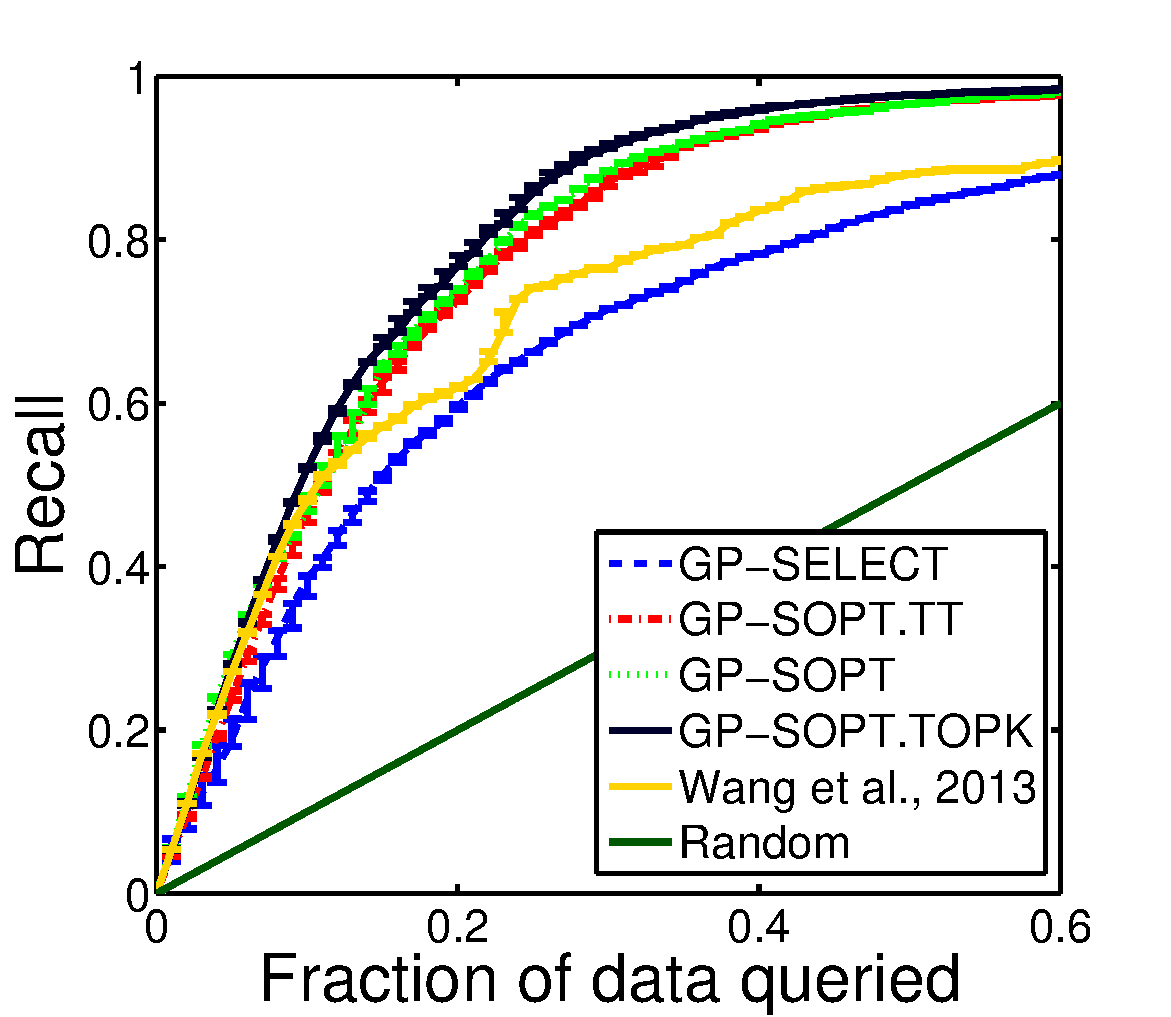
\includegraphics[width=0.31\textwidth,height=0.25\textwidth]{../exp/final_results/populated_places_5000_result_5seeds_top15p_omega0-001_lapnorm0_new.pdf}} &
\subfigure[Wikipedia]{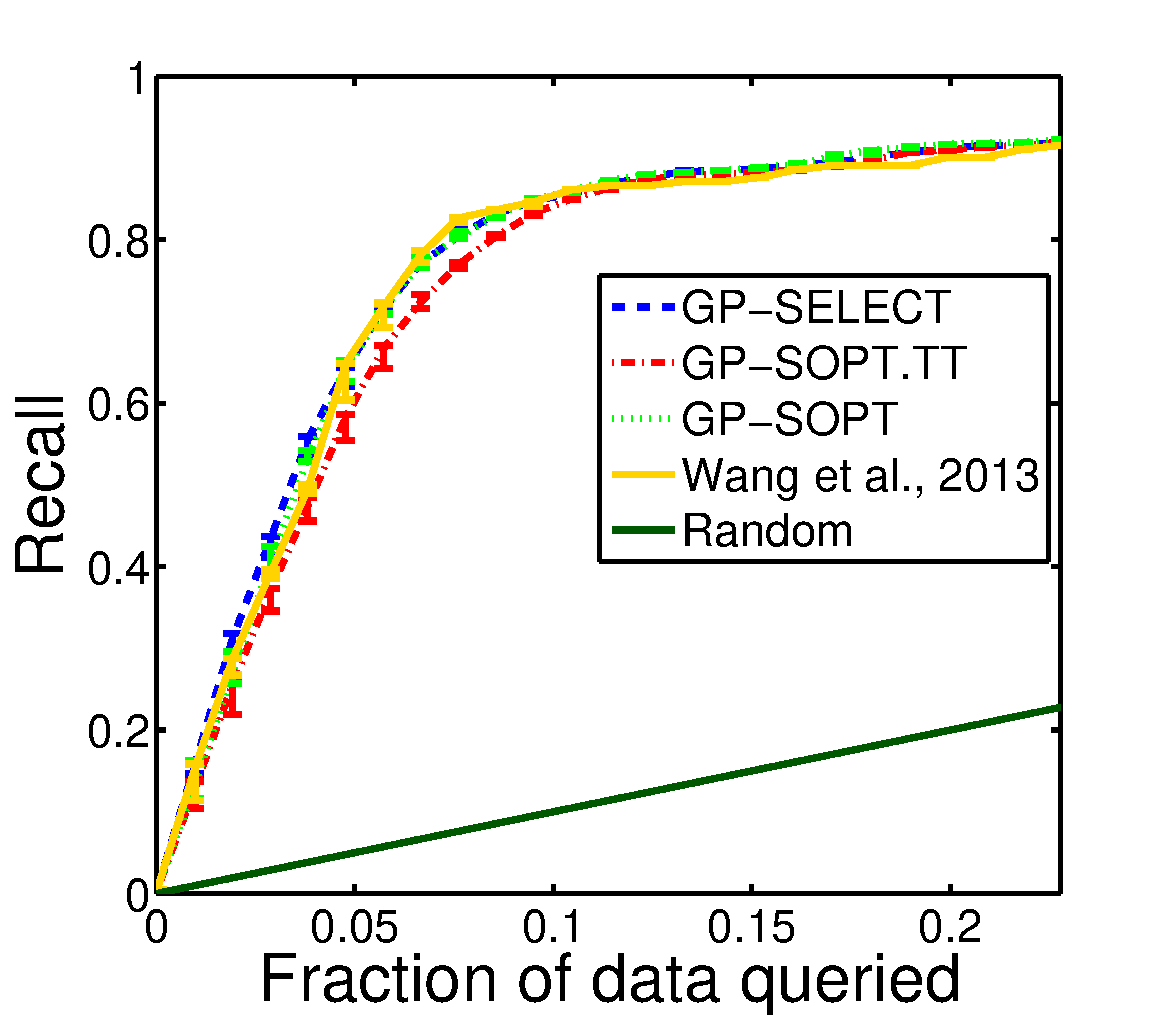
\includegraphics[width=0.31\textwidth,height=0.25\textwidth]{../exp/final_results/wiki_result_5seeds_top15p_omega0-001_lapnorm0_new.pdf}} &
\subfigure[Citation Network]{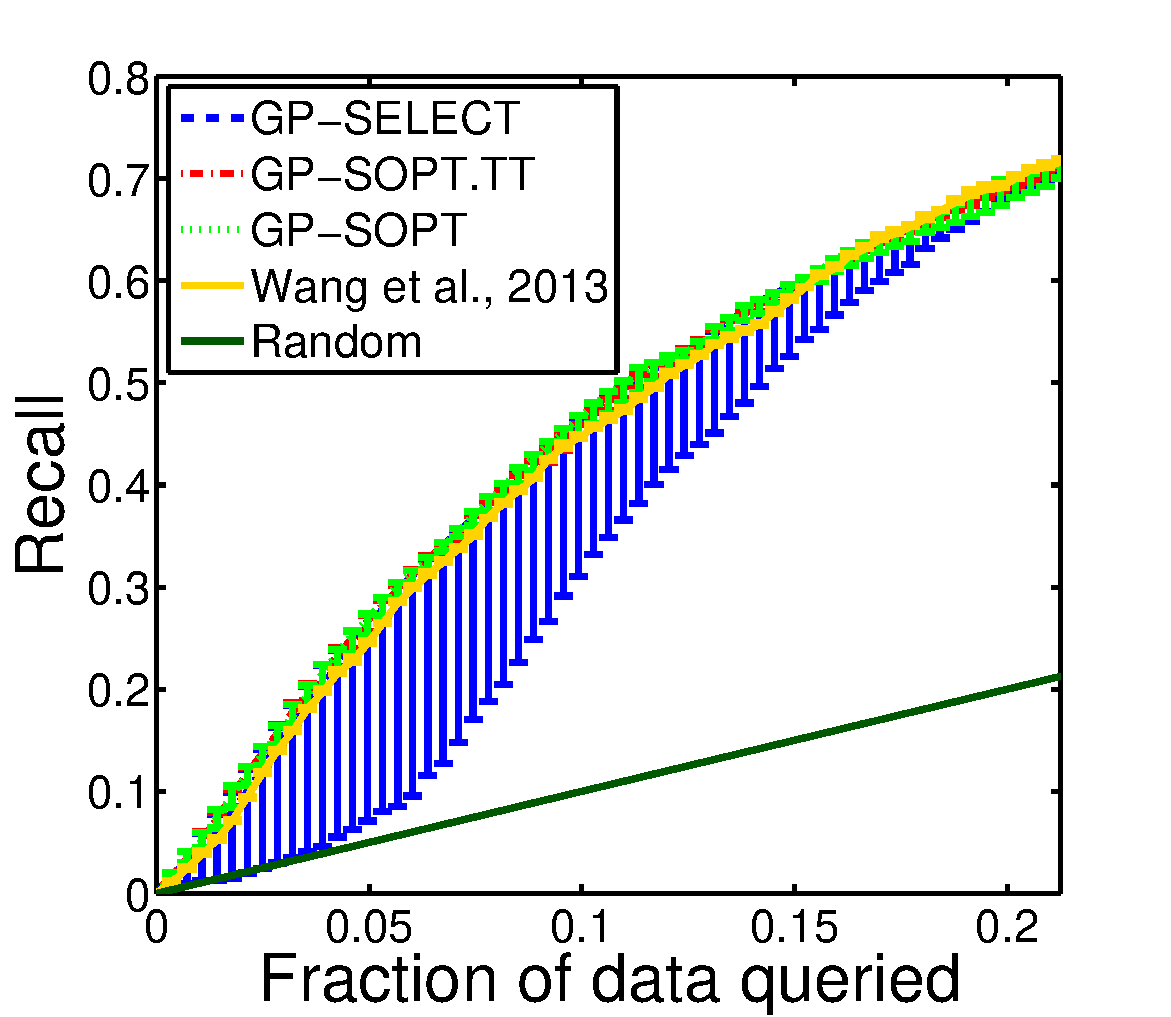
\includegraphics[width=0.31\textwidth,height=0.25\textwidth]{../exp/final_results/new_nips_result_5seeds_top15p_omega0-001_lapnorm0.pdf}}
\end{tabular}
\end{center}
\caption{Recall vs. fraction of data queried}
\label{fig:results}
\end{figure*}
We conduct experiments on three graph data sets that were studied by \cite{wang2013active}
and a version of the Enron e-mail data by \cite{enron}.
\subsection[Three Graph Datasets of Wang et al., 2003]{Three Graph Datasets of \cite{wang2013active}}
We briefly summarize the datasets below.

\textbf{5000 Populated Places.} The nodes of this graph are 5000 concepts in the DBpedia\footnote{www.dbpedia.org} ontology marked as populated places.
Each place is supported by a Wikipedia page, and an undirected edge is created between two 
places if either one of their two Wikipedia pages links to the other. There can be multiple 
edges between two places. The DBpedia 
ontology divides populated places into five categories: administrative regions, countries, cities, towns and villages.
The 725 administrative regions are selected as our target class while all the others are considered to be in null class.   
  
\textbf{Citation Network.} This dataset consists of 14,117 papers in top Computer Science venues available on citeseer. 
The graph is created by adding an undirected edge between two papers if either one cites the other. The 1844 NIPS papers
are chosen as our target class. 

\textbf{Wikipedia Pages on Programming Languages.} A total of 5,271 Wikipedia pages related to programming languages are the nodes 
of this graph, and an undirected edge exists between two pages if they are linked together. \cite{wang2013active} performed topic 
modeling and chose the 202 pages related to objective oriented programming as our target class.
%, treating all the others as null class.   
 
As demonstrated by \cite{wang2013active}, the three graphs and their target label distributions exhibit qualitative differences
and thus serve as good benchmarks. The citation network has many small components and target nodes appear in many of them, 
while the Wikipedia graph has large hubs and most target nodes reside in one of them. 
The graph of populated places lies in between these two extremes, with components of various sizes containing target nodes.   

On all of the three data sets we compare two of the proposed methods: GP-SOPT.TT and GP-SOPT against GP-SELECT (GP-UCB without replacement) 
and the active search algorithm (AS-on-Graph) by \cite{wang2013active}. We only evaluate GP-SOPT.TOPK on the 5000 populated places data
due to its heavy computation. For each dataset we perform 5 independent runs, each with a randomly
chosen target node as the warm start seed. 
For the proposed methods and GP-SELECT, the main tuning parameters  
are the exploration-exploitation trade-off parameter $\alpha_t$ and the observation noise variance $\sigma^2$.
For GP-SOPT.TT and GP-SOPT.TOPK there is additionally the thresholding parameter $k$. 
We consider the following values for them. 
Populated Places: $\alpha_t \in \{4,2,1,0.1,0.01,0.001\}$, $\sigma^2 \in \{1,0.5,0.25,0.1\}$ and $k \in \{200,400,800\}$. 
Wikipedia: $\alpha_t \in \{0.1,0.01,0.001\}$, $\sigma^2 \in \{1,0.5,0.25,0.1\}$ and $k \in \{200,400,800\}$.  
Citation Network: $\alpha_t \in \{1,10^{-1},10^{-2},10^{-3},10^{-4}\}, \sigma^2 \in \{1,0.5,0.25,0.1\}$ and  $k \in \{400,800,1600\}$.
Although in theory $\alpha_t$ should be iteration-dependent, we find that a fixed value often performs well in practice.
On all data sets we set the kernel regularization parameter $\omega_0 = 0.01$.
\cite{wang2013active} algorithm has several parameters, and we only tune the exploration-exploitation trade-off parameter $\alpha$. It is set to 0.1 on Populated Places and Citation Network,
and 0.0001 on Wikipedia, which are the best performing values. Other parameters are set based on \cite{wang2013active}. 


Results are in  Figure~\ref{fig:results}, where we plot the recall, i.e., the fraction of 
targets found by the algorithms, versus the fraction of the whole data set queried.
More specifically, for each algorithm we obtain its mean recall curve over the top 15\% (except for \cite{wang2013active})
parameter combinations in each experiment, as judged by the area under the recall curve.
We then plot the median, maximum and minimum over the five runs in Figure~\ref{fig:results}.

The three proposed methods clearly outperform \cite{wang2013active} and GP-SELECT on Populated Places, while all methods 
perform equally well on Wikipedia. We think this has to do with the underlying graph structure and target distribution.
As mentioned before, target nodes in the Populated Places graph are spread over sub-graphs of various sizes, and therefore exploration strategies 
do make a difference. We observe that the proposed methods tend to select high-degree nodes in the first few iterations, thereby
gaining much information, while GP-SELECT initially selects low-degree nodes.  
In contrast, most target nodes in the Wikipedia graph reside in one large component, and therefore 
less exploration is needed. In fact, the best values for $\alpha_t$ are very small, suggesting that an exploitation-only 
strategy is good enough for this data. On Citation Network, most methods perform well except that GP-SELECT performs 
quite poorly in one run. This may again indicate GP-SELECT is less robust against low-degree nodes. 
\subsection{Enron E-mails}
We experimented on the Enron e-mail data set\footnote{Available at \url{http://cis.jhu.edu/~parky/Enron/execs.email.linesnum.ldctopic} \label{note:enron}} 
with topics assigned by \cite{enron} based on the annotations by \cite{enron_topics}. 
We further processed the dataset into a format suitable for active search experiments as detailed below. 
Each e-mail $i$ is represented by a unique Unix time stamp $t_i$, a unique sender index and the set of receiver (excluding self-copying) indices, which are collectively 
denoted as $U_i$. Between e-mails $i$ and $j$, we created an edge with the following weight:

\centerline{
$A_{ij} :=  \exp\left( - (t_i - t_j)^2 / \tau^2 \right) \cdot |U_i \cap U_j| / \sqrt{|U_i||U_j|}$,	
}

where $\tau = 12$ weeks in seconds and $|U_i|$ denotes the size of $U_i$. 
We thus measure pairwise similarity among e-mails by the product of 
nearness in time and degree of overlap between users involved. 
The resulting e-mail graph has 20,112 nodes, and we chose the subset of 803 e-mails that are assigned topic 16 in LDC topics\footnoteref{note:enron}, 
which is related to the downfall of Enron, to be the target class in this experiment.

Due to the size of the dataset, we only compared three methods: GP-SOPT.TT, GP-SELECT and \cite{wang2013active}
in three independent runs each initialized with a target node chosen uniformly at random.
We also limited the tuning parameters to be the following fixed values across the three runs:
$(k,\alpha,\sigma^2,\omega_0) = (800, 0.001, 0.05, 0.01)$ for GP-SOPT.TT, $(\alpha, \sigma^2, \omega_0) = (0.01, 0.05, 0.01)$ for GP-SELECT, 
and $\alpha = 0.001$ for \cite{wang2013active}. These values were chosen based on a coarse parameter search to be indicative of the performance of each method on this data set.
\begin{figure}[t]
\centering
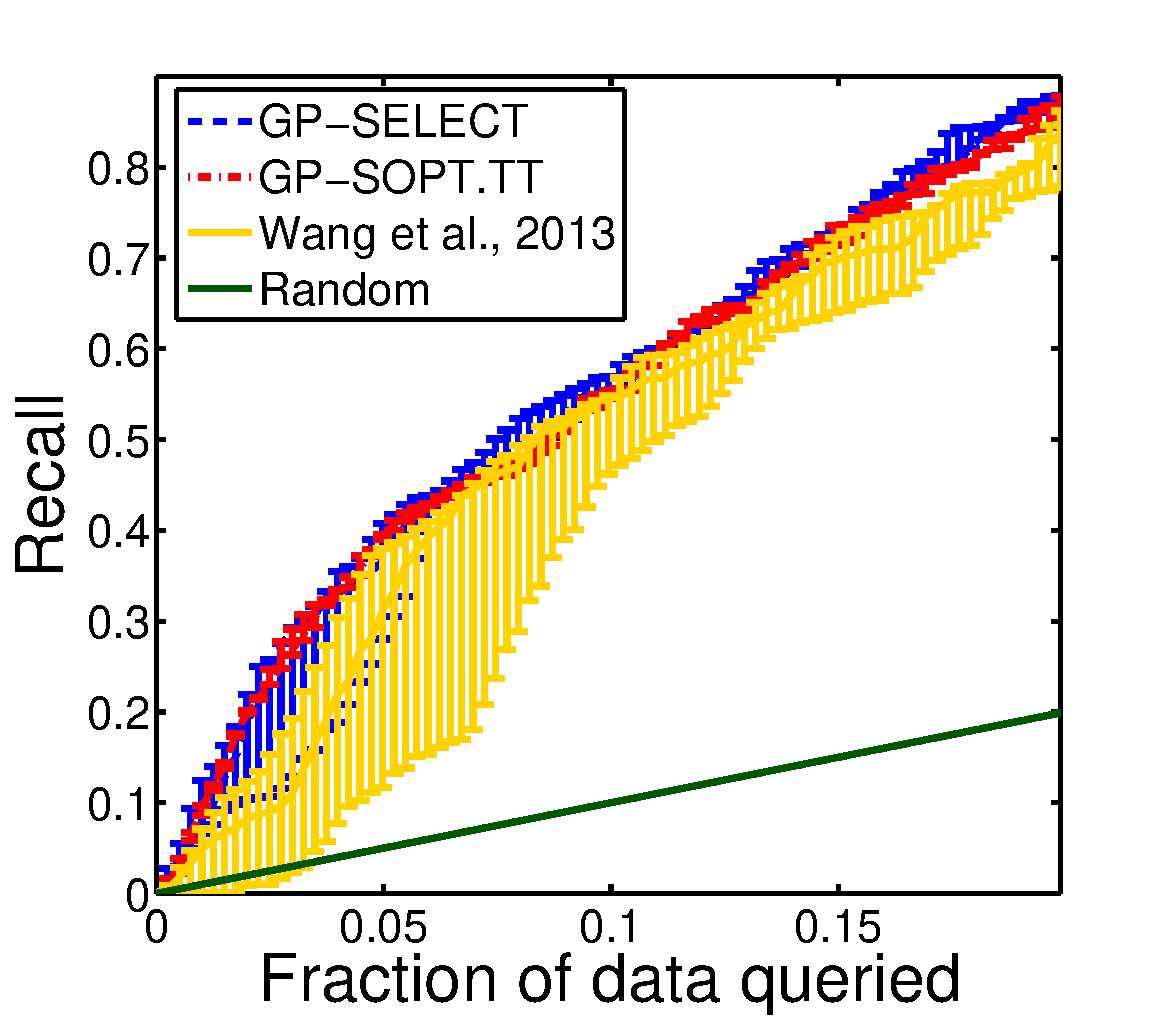
\includegraphics[width=0.31\textwidth,height=0.25\textwidth]{../exp/final_results/enron.pdf}
\caption{Enron: recall vs. fraction of data queried}
\label{fig:enron}
\end{figure}
Results are in Figure~\ref{fig:enron}, which shows GP-SOPT.TT is more stable across initial seeds than the other methods, and outperforms \cite{wang2013active} significantly at early iterations. 


%%%%%%%%%%%%%%%
\section{CONCLUSION AND DISCUSSIONS}
\label{sec:conclude}

In this paper, we discuss active search on a graph with known structure. Each node bears a reward, which is unknown at first but can be noisily observed upon query. 
An active search algorithm aims to accumulate as large a sum of rewards from the queried nodes as possible under limited budgets. 
We assume that the node rewards vary smoothly along the graph.

Popular Bayesian UCB-style algorithms \citep{srinivas2012information,vanchinathanadaptively,valko2014spectral}
use the marginal standard deviation as their exploration criterion, leading to the undesirable tendency
of selecting peripheral nodes on a graph. Instead, we consider 
$\Sigma$-optimality on graphs, which can more efficiently reduce the variance of the reward function estimate by 
sampling cluster centers. We show the advantage of our method in experiments with real graphs and 
provide a theoretical guarantee on the cumulative regret.


One interesting future direction is deriving tighter regret bounds for the proposed methods that match their empirical performances. 
%Our earlier version contained a theoretical result with better rates; unfortunately it was found to be incorrect because it used proof strategies from \cite{contal2014gaussian} that contained mistakes.
We imagine it may be possible to bound the regret directly by the difference in $\Sigma$-optimality (Bayes survey risks, $\mathcal{R}^{\Sigma}$), which may have better properties than differential information gain, $\gamma_T$ on graphs.

An equally interesting question is the selection of graph kernels. Our discussions and experiments mainly consider Gaussian random fields with unnormalized Laplacian, which is a very popular kernel choice. 
It is worthwhile to 
%Different kernels and regularizations may result in different performances of the same algorithm. 
explore active search with other graph kernels, such as the ones discussed in \cite{SmolaK03}.


\subsubsection*{Acknowledgement}
This work was funded in part by DARPA grant FA87501220324.

\appendix

%\input{appendix_spectral_ucb_equivalence.tex}
% \input{appendix_covariance_nonnegative.tex}
% !TEX root = as_grf_sopt.tex

% \begin{appendices}


\section{Predictive Covariance Matrix}
\label{sec:appendix:cov}

   
   
   
   
%%%%%%%%%%%%
\begin{lemma}
\label{lemma:nnC} 
  For augmented graph Laplacian, %$\bC=(\cLap+\omega_0\bI)$,
  the posterior covariance matrix, $C_t(v,v')\geq0, \forall v, v'$.
\end{lemma}%
\begin{proof}
  Let $h_k = \sum_{\tau=1}^t e_{v_\tau}(v_k)$ to be the count of queries on node $k$; further define its diagonal matrix, $\bH = \diag(h_1,\dotsc,h_n)$. 
  We rewrite \eqref{eq:post_prec} as, %The conjugate inference model in term of the precision matrix is,
\begin{equation*}
    (\bC_t)^{-1} = (\bC_0)^{-1} + \sigma_n^{-2}\bH
    = \bD - \bA + \omega_0\bI + \sigma_n^{-2}\bH
  \end{equation*}
  Define $\bD_t = \bD + \omega_0\bI + \sigma_n^{-2}\bH$,
  we have
  \begin{align*}
    \bC_t = (\bD_t - \bA)^{-1}
    =
    \bD_t^{-\frac{1}{2}}
    \left(\sum_{k=0}^\infty \left(\bD_t^{-\frac{1}{2}}\bA\bD_t^{-\frac{1}{2}}\right)^k \right)
    \bD_t^{-\frac{1}{2}}, 
  \end{align*}
where the right hand side is always nonnegative.

%%%%%%%%%%%%%
The convergence of $\|\bD_t^{-\frac{1}{2}} \bA \bD_t^{-\frac{1}{2}}\|_2 < 1$ is as follows.
%Assume $\sigma_n^2>0$, show  $\|\bD_t^{-\frac{1}{2}} \bA \bD_t^{-\frac{1}{2}}\|_2 < 1$.

Define the components for the posterior as $\bD_t = \diag(d_1^{(t)}, \dotsc, d_n^{(t)}$ with $d^{(t)} = \sum_{i=1}^n d_i^{(t)}$. Also, define for the prior model $\bD = \diag(d_1^{(0)}, \dotsc, d_n^{(0)}$ with $d^{(0)} = \sum_{i=1}^n d_i^{(0)}$.

The following holds for any $\bv\in\mathbb{R}^n$,
\begin{align*}
	&\quad \bv^\top \bD_t^{-\frac{1}{2}} \bA \bD_t^{-\frac{1}{2}} \bv 
	= \sum_{ij}\frac{v_i v_j a_{ij}}{\sqrt{d^{(t)}_i}\sqrt{d^{(t)}_j}}
	\\
	&\leq 
	\sqrt{
		\left(  \sum_{ij} \frac{v_i^2 a_{ij}}{d^{(t)}_i}  \right)
		\left(  \sum_{ij} \frac{v_j^2 a_{ij}}{d^{(t)}_j}  \right)
	}
	=\sum_i v_i^2 \frac{d_i}{d^{(t)}_i}
	\leq \|\bv\|_2^2.
\end{align*}

Further, both equalities cannot hold simultaneously, because for the first equality to hold, it is required that $\frac{v_i^2a_{ij}}{d_i^{(t)}} \propto \frac{v_j^2a_{ij}}{d_j^{(t)}}$, i.e., $v_j^2 \propto d_j^{(t)}, \forall j$ in the same connected component, which then dictates that,
\begin{align*}
	\sum_i v_i^2 \frac{d_i}{d^{(t)}_i} 
	= \sum_i \left( \frac{d_i^{(t)}}{d^{(t)}} \|\bv\|_2^2\right) \frac{d_i}{d^{(t)}_i}
	= \frac{ d^{(0)} }{ d^{(t)} }\|\bv\|_2^2 
	<\|\bv\|_2^2.
\end{align*}
\end{proof}


%
%%%%%%%%%%%%%
%\begin{remark}
% Notice that Lemma~\ref{lemma:nnC} also applies to normalized graph Laplacians, when because the counterpart of \eqref{eq:precision} allows a similar derivation,
% \begin{align*}
%   \widetilde{\bC}_t 
%   &= 
%   \left( \widetilde{\cLap} +
%   \widetilde{\bOmega} + \sigma_n^{-2}\bH
%   \right)^{-1} 
%   \numberthis
%   \label{eq:nnC_normalized}
%   \\
%%    &=
%%    \bD^{\frac{1}{2}}
%%    \left( \bD - \bA 
%%    + \widetilde{\bOmega}\bD + \sigma_n^{-2}\bH\bD
%%    \right)^{-1}
%%    \bD^{\frac{1}{2}},
%%    \\
%   &=
%   \bD^{\frac{1}{2}}
%   \widetilde{\bD}^{-\frac{1}{2}}
%   \left( \sum_{k=0}^\infty \left(
%     \widetilde{\bD}_t^{-\frac{1}{2}} 
%     \bA
%     \widetilde{\bD}_t^{-\frac{1}{2}} 
%   \right)^k
%   \right)^{-1}
%   \widetilde{\bD}^{-\frac{1}{2}}
%   \bD^{\frac{1}{2}},
% \end{align*}
% when the counterpart of $\bD_t$ is defined as,
% \begin{equation}
%   \widetilde{\bD}_t = \bD + \widetilde{\bOmega}\bD + \sigma_n^{-2}\bH\bD.
% \end{equation}
% Generally we require $\sigma_n > 0$, but it is not necessary for submatrix of covariance matrix on unqueried nodes (more in Appendix~\ref{app:sec:nnC}).
%\end{remark}
%

%%%%%%%%%%%%%

%\begin{lemma}
%If  prior is defined with respect to an unnormalized graph Laplacian, we have for any $t$ and $(v,v')$ pair, 
%\begin{equation}
%  C_t(v,v) \geq C_t(v,v'),
%\end{equation}
%which essentially means $\sigma_t(v) \geq \rho_t(v,v')\sigma_t(v'), \forall v'$.
%\end{lemma}%
%%%%%%%%%%%%%%%%
%
%We can use spring analogy in spectral graph models, which assumes that the nodes are physical particles that can move vertically. Two particles $v,v'$, are connected with springs of strength $A(v,v')$, if the weight is nonnegative. Every node is also connected to a reference point (assuming that to be of level zero) with spring of strength $\omega_0+\frac{h_v}{\sigma_n^2}$. 
%  
%  In this analogy, the displacement of a node $v$ in height by applying unit form is proportional to $C(v,v)$, whereas the vertical displacement of another node $v'$  by applying unit force on node $v$ is $C(v,v')$. For a trivial example, imagine $A=0$ and displacement, inversely related to the spring strength, is exactly $(\omega_0+\frac{h_v}{\sigma_n^2})^{-1}$. From physical models, we can observe that the displacement of any other node is always smaller than self-displacement, when force is applied. 
%\end{proof}

\begin{lemma}
\label{lemma:nnC_sub}	
The diagonal elements in $\bC_t$ is always no smaller than the off-diagonal elements, i.e., $\sigma_t(v)^2 = C_t(v,v)\geq C_t(v,v'), \forall v,v'$.
% Let $C$ denote the posterior covariance conditioned on a set $S$ of nodes. For any $U \subset V \setminus S$, we have
% that $C_{U,U}$ is non-negative elementwise.
\end{lemma}


\newcommand{\bbv}{\bar{\bv}}
\newcommand{\bell}{\boldsymbol{\ell}}

\begin{proof}
	Without loss of generality, let $v$ be the last index of $\bC_t=(\widetilde{\cLap}_0 + \sigma_n^{-2}\bH)^{-1}$. For simplicity, let $\widetilde{\cLap}_t = \widetilde{\cLap}_0 + \sigma_n^{-2}\bH$ and it has the following matrix partition,
	\begin{equation*}
		\widetilde{\cLap}_t
		= \begin{pmatrix}
			\widetilde{\cLap}_{\bbv \bbv} & \tilde{\bell}_{\bbv v}
			\\
			\tilde{\bell}_{\bbv v}^\top & \tilde{\ell}_{vv}
		\end{pmatrix},
	\end{equation*}
	where $\bbv$ is the complement of $v$.
	From Woodbury matrix inversion lemma, we have
	\begin{equation}
		\bC_t = \widetilde{\cLap}_t^{-1}
		= \begin{pmatrix}
			\mathbf{M}
			 &
			-\frac{1}{m}
			\widetilde{\cLap}_{\bbv\bbv}^{-1} \tilde{\bell}_{\bbv v}
			\\
			-\frac{1}{m}
			\tilde{\bell}_{\bbv v}^\top \widetilde{\cLap}_{\bbv\bbv}^{-1}
			&
			\frac{1}{m}
		\end{pmatrix},	
	\end{equation}
	where $m=\tilde{\ell}_{vv} - \tilde{\bell}_{\bbv v}^\top \widetilde{\cLap}_{\bbv\bbv}^{-1} \tilde{\bell}_{\bbv v} $
	and $\mathbf{M}=
			 \widetilde{\cLap}_{\bbv\bbv}^{-1}+\frac{1}{m} 
			 \widetilde{\cLap}_{\bbv\bbv}^{-1} \tilde{\bell}_{\bbv v}
			 \tilde{\bell}_{\bbv v}^\top \widetilde{\cLap}_{\bbv\bbv}^{-1}
	$.
	To show that $C_t(v,v)\geq C_t(v,v')$, we need to verify that 
$
	(			-\widetilde{\cLap}_{\bbv\bbv}^{-1} \tilde{\bell}_{\bbv v}
)_{v'}\leq1.
$

	In fact, since $\widetilde{\cLap}_t
	%=\widetilde{\cLap}_0+\sigma^{-2}\bH
	$ is diagonally dominant, we have
	$\widetilde{\cLap}_t \bone_n\geq0.
	$
	Take its first $n-1$ rows to get
	$
		\widetilde{\cLap}_{\bbv \bbv}\cdot \bone_{n-1} +
		\tilde{\bell}_{\bbv v} \geq 0.
	$
	Notice $\widetilde{\cLap}_{\bbv \bbv}$ is also a valid augmented graph Laplacian. By Lemma \ref{lemma:nnC}, we could left multiply the element-wise nonnegative matrix $\widetilde{\cLap}_{\bbv \bbv}^{-1}$ to both sides to obtain,
$		\bone_{n-1} +
		\widetilde{\cLap}_{\bbv \bbv}^{-1}\tilde{\bell}_{\bbv v} \geq 0,
$
	which completes our proof for any $v'\in \bbv$.
\end{proof}

% \begin{proof}
% 	Let $\tilde{L} := L + \omega_0 I$.
% Suppose the prior covariance matrix decomposes into,
% \begin{equation}
% 	K \;=\; 
% 	\begin{bmatrix}
% 		\tilde{L}_{S,S}  & \tilde{L}_{S,U} \\
% 		\tilde{L}_{U,S} & \tilde{L}_{U,U}
% 	\end{bmatrix}^{-1}.
% \end{equation}
% Schur complement then gives
% \begin{align}
% 	K_{S,S} &= (\tilde{L}_{S,S} - \tilde{L}_{S,U} (\tilde{L}_{U,U})^{-1}\tilde{L}_{U,S})^{-1},\\
% 	K_{U,U} &= (\tilde{L}_{U,U})^{-1}( I + \tilde{L}_{U,S} K_{S,S} \tilde{L}_{S,U} (\tilde{L}_{U,U})^{-1}),\\
% 	K_{S,U} &= -K_{S,S} \tilde{L}_{S,U} (\tilde{L}_{U,U})^{-1}.
% \end{align}
% By conjugate inference formula, we have
% \begin{align}
% 	C_{S,S} &= K_{S,S} - K_{S,S}(K_{S,S}+\sigma^2 I)^{-1}K_{S,S}\\
%                 &= (\sigma^{-2}I + K_{S,S}^{-1})^{-1}\\
% 			      & = (\tilde{L}_{S,S} + \sigma^{-2} I- \tilde{L}_{S,U} (\tilde{L}_{U,U})^{-1}\tilde{L}_{U,S})^{-1}, \label{eq:C_SS}\\
% 	C_{U,U} 
% 	&= K_{U,U} - K_{U,S}(K_{S,S} + \sigma^2 I)^{-1} K_{S,U}\\
% 	&= (\tilde{L}_{U,U})^{-1}(I + \tilde{L}_{U,S}C_{S,S}\tilde{L}_{S,U}(\tilde{L}_{U,U})^{-1}).
% \end{align}
% Plugging \eqref{eq:C_SS} into \eqref{eq:C_UU} and applying the matrix inversion lemma, we get
% \begin{equation}
% 	C_{U,U} = (\tilde{L}_{U,U} - \tilde{L}_{U,S}(\tilde{L}_{S,S} + \sigma^{-2}I)^{-1}\tilde{L}_{S,U})^{-1}.
% \label{eq:C_UU}
% \end{equation}
% Again by Schur complement, we get
% \begin{equation}
% 	C_{U,U} = (\bar{L}^{-1})_{U,U},
% \end{equation}
% where
% \begin{equation}
% 	\bar{L} :=
% 	\begin{bmatrix}
% 		\tilde{L}_{S,S} + \sigma^{-2}I & \tilde{L}_{S,U} \\
% 		\tilde{L}_{U,S} & \tilde{L}_{U,U}
% 	\end{bmatrix}.
% \end{equation}
% Because $\bar{L}$ satisfies Proposition 6 of \cite{ma_2013}, $\bar{L}^{-1}$ is non-negative elementwise, and so is $C_{U,U}$.
% \end{proof}


% In fact, this Lemma can be applied to also labeled nodes by constructing an auxiliary ``labeled node'' that connects to every other node with weight equal to the regularization parameter of that node.

% \end{appendices}

%\input{appendix_better_proofs.tex}
% !TEX root = as_grf_sopt.tex

% \begin{appendices}
\section{Active Search Regret Bound}
\label{appendix:proof_as_regret}
We start by stating the following result.% by \cite{srinivas2012information}.
\begin{theorem}[Theorem 6, {\cite{srinivas2012information}}]
	\label{thm:dev}
	Let $\delta \in (0,1)$. Assume the observation noises are uniformly bounded by $\sigma_n$ and $f$ has RKHS norm $B$ with kernel $C_0$, which is equivalent to $\bff^\top\widetilde{\cLap}_0\bff\leq B^2$. Define 
	% \begin{equation*}
	$
		\alpha_t = \sqrt{2 B^2 + 300 \gamma_t \log(t/\delta)^3},
		$
	% \end{equation*}
	% where $\Vert \cdot \Vert_K$ denotes the RKHS norm associated with the kernel $K$. Then
	then
	\begin{equation*}
		\mbox{Pr}\left(\forall t, \forall v \in V, \;\; |\mu_t(v) - f(v)| \leq \alpha_{t+1} \sigma_t(v) \right) \geq 1 - \delta.
	\end{equation*}
\end{theorem}
We use this result to bound our instantaneous regrets.
\begin{lemma}
	Conditioned on the high-probability event in Theorem \ref{thm:dev}, the following bound holds:
	\begin{equation*}
		\forall t, \;\; r_t := f(v^*_t) - f(v_t) \leq 2 \alpha_t k \sigma_{t-1}(v_t), 
	\end{equation*}
	where $v^*_t$ is the node with the $t$-th globally largest function value and $v_t$ is node selected at round $t$. 
\end{lemma}
%\begin{proof}
\emph{Proof}.
At round $t$ there are two possible situations. If 
$v^*_t$ was picked at some earlier round, the definition of $v^*_t$ implies that there exists some $t' < t$ such that $v^*_{t'}$ 
has not been picked yet. According to our selection rule, the fact that $s_t(v) \geq \sigma_t(v)$, 
and Theorem \ref{thm:dev}, the following holds:
\begin{align*}
	&\mu_{t-1}(v_t) + \alpha_t s_{t-1}(v_t) \geq \mu_{t-1}(v^*_{t'}) + \alpha_t s_{t-1}(v^*_{t'}) \\
		&\qquad \geq \mu_{t-1}(v^*_{t'}) + \alpha_t \sigma_{t-1}(v^*_{t'})
	 \geq f(v^*_{t'}) \geq f(v^*_t).
\end{align*}
If $v^*_t$ has not been picked yet, a similar argument gives 
\begin{equation*}
	\mu_{t-1}(v_t) + \alpha_t s_{t-1}(v_t) \geq \mu_{t-1}(v^*_{t}) + \alpha_t s_{t-1}(v^*_{t}) 
		%&\geq& \mu_{t-1}(v^*_{t}) + \alpha_t \sigma_{t-1}(v^*_{t})\\
	\geq f(v^*_t).
\end{equation*}
Thus we always have 
\begin{align*}
f(v^*_t) &\leq \mu_{t-1}(v_t) + \alpha_t s_{t-1}(v_t) \\
&\leq f(v_t) + \alpha_t \sigma_{t-1}(v-t) +\alpha_t s_{t-1}(v_t)\\
%&\leq& f(v_t) + 2 \alpha_t s_{t-1}(v_t) \\
&\leq f(v_t) + 2 \alpha_t k \sigma_{t-1}(v_t).	
\end{align*}
%\end{proof}
%\begin{lemma}[Lemma 5.3, {\cite{srinivas2012information}}]
%	The information gain achieved by the selected nodes can be expressed in terms of the predictive variances.
%	Let $\bv_t = (v_1, v_2, \ldots, v_t)$ denote the sequence of selected nodes. Then
%	\begin{equation*}
%		\mathcal{I}(\by_{\bv_t};f_{\bv_t}) = \frac{1}{2} \sum_{i=1}^t \log(1 + \sigma^{-2}\sigma_{i-1}(v_i)^2). 
%	\end{equation*}
%\end{lemma}
%Next we bound the sum of squared instantaneous regrets in terms of the maximum information gain. 
\begin{lemma}[Lemma 5.4, {\cite{srinivas2012information}}]
	Let $\alpha_t$ be defined as in Theorem \ref{thm:dev} and $c_1$ be defined as in Theorem \ref{thm:as_regret}.
	Conditioned on the high probability event of Theorem \ref{thm:dev}, the following holds:
	\begin{equation*}
	\forall T\geq 1, \;\;\sum_{t=1}^T r_t^2 \leq \alpha_T k^2 c_1 \mathcal{I}(\by_{\bv_T};f_{\bv_T}) \leq \alpha_T k^2 c_1 \gamma_T.	
	\end{equation*}
\end{lemma}
Finally, the Cauchy-Schwarz inequality gives  
$R_T \leq \sqrt{T \sum_{t=1}^T r_t^2} \leq k \sqrt{T c_1 \alpha_T \gamma_T}.$
% \end{appendices}

% \input{appendix_Cprime_opt_regret.tex}
%\input{appendix_proof_opt_regret.tex}


\renewcommand\bibsection{\subsubsection*{References}}
\bibliographystyle{plainnat}
\bibliography{myrefs}




\end{document}
